\chapter{DeepSeek: The Final Adventure}

\section{Introduction: The Quest for Efficient Attention}

In the previous chapter, we explored the evolution of transformer inference optimizations, from the foundational Key-Value (KV) Cache to the memory-saving innovations of Multi-Query Attention (MQA) and Grouped Query Attention (GQA). We saw how these techniques dramatically reduced the computational and memory overhead of large language models, enabling longer context windows and faster inference. Yet, as we push the boundaries of what language models can do, a fundamental question remains: \textit{Can we achieve even greater efficiency without sacrificing model performance?}

This question lies at the heart of DeepSeek's breakthrough. As we have seen, the KV cache is a double-edged sword: it accelerates inference by avoiding redundant computation, but its memory requirements can quickly become prohibitive as models and context windows scale. MQA and GQA offer clever compromises, trading off some expressive power for memory savings by sharing key and value matrices across heads or groups of heads. However, these approaches inevitably limit the diversity of information each attention head can capture, leading to a drop in model performance, especially on tasks requiring nuanced understanding.

\textbf{The challenge is clear:} We want the best of both worlds---the low memory footprint of MQA, and the rich, diverse representations of standard Multi-Head Attention (MHA). Is it possible to design an attention mechanism that is both memory-efficient and highly expressive?

\subsection{The Road So Far: A Recap}

Let us briefly recap the journey that has brought us here:

\begin{itemize}
    \item \textbf{KV Cache} transformed inference by storing previously computed keys and values, reducing redundant computation and making long-context inference feasible. But its memory cost grows linearly with the number of layers, heads, head dimension, and context length.
    \item \textbf{Multi-Query Attention (MQA)} slashed memory usage by sharing a single set of keys and values across all heads, but at the cost of reduced diversity among attention heads.
    \item \textbf{Grouped Query Attention (GQA)} struck a balance, sharing keys and values within groups of heads, offering a middle ground between memory savings and model expressiveness.
\end{itemize}

Despite these advances, a tension remains: as we reduce the number of unique key-value sets, we also reduce the model's ability to capture complex, multi-faceted relationships in language. The trade-off between efficiency and expressiveness seems inescapable.

\subsection{The Need for a New Paradigm}

This is where DeepSeek's innovation---\textbf{Multi-Head Latent Attention (MLA)}---enters the story. The DeepSeek team asked a bold question: \textit{Can we rethink the very structure of the attention mechanism to break the trade-off between memory and performance?}

Their answer is both elegant and profound. By introducing a shared latent space and leveraging mathematical absorption tricks, MLA allows the model to cache a single, compact latent matrix instead of separate key and value matrices for each head. This approach not only slashes the memory requirements by an order of magnitude, but also preserves---and in some cases even enhances---the diversity and power of multi-head attention.

In the further sections, we will embark on a detailed exploration of Multi-Head Latent Attention (MLA). We will build on the foundations laid in previous chapters, revisit the limitations of existing approaches, and step by step, uncover the intuition, mathematics, and practical implementation of MLA. Our goal is to demystify this innovation, showing not just how it works, but why it represents a fundamental leap forward in efficient transformer design.

Let us begin our journey into the world of DeepSeek and the next frontier of attention mechanisms.

\section{Multi-Head Latent Attention: Concept and Process Flow}

As we seek to break the trade-off between memory efficiency and model expressiveness, DeepSeek's Multi-Head Latent Attention (MLA) introduces a fundamentally new approach. Instead of caching separate key and value matrices for each attention head, MLA proposes to cache a single, compact latent matrix---dramatically reducing memory requirements while preserving the diversity of attention heads.

\subsection{The Motivation: Reducing the KV Cache}

Recall the formula for the size of the KV cache in standard multi-head attention:
\begin{equation}
\text{Size of KV cache} = l \times b \times n \times h \times s \times 2 \times 2 \label{eq:kv_cache_size}
\end{equation}
where:
\begin{itemize}
    \item $l$: number of transformer layers
    \item $b$: batch size
    \item $n$: number of attention heads
    \item $h$: head dimension
    \item $s$: context length (number of tokens)
    \item $2$: for keys and values
    \item $2$: bytes per parameter (assuming 16-bit precision)
\end{itemize}

DeepSeek's goal is to reduce the dominant term from Equation \eqref{eq:kv_cache_size}:
\begin{equation}
2 \times n \times h \longrightarrow d_L \label{eq:reduction_goal}
\end{equation}
where $d_L$ is a much smaller latent dimension. To achieve this, DeepSeek projects the input embedding matrix into a lower-dimensional latent space.

\subsection{The Latent Projection: Building the Latent Matrix}

Given input embedding matrix $X \in \mathbb{R}^{\text{batch\_size} \times s \times d_{\text{model}}}$:

\begin{enumerate}
    \item \textbf{Project to Latent Space with LayerNorm:}
    \begin{equation}
    C_{\text{KV}} = \text{LayerNorm}(X W_{\text{DKV}}) \label{eq:simple_ckv}
    \end{equation}
    where $W_{\text{DKV}} \in \mathbb{R}^{d_{\text{model}} \times d_L}$, so $C_{\text{KV}} \in \mathbb{R}^{\text{batch\_size} \times s \times d_L}$. This is the latent matrix we cache.

    \item \textbf{Compute Queries:}
    \begin{equation}
    Q = X W_Q \label{eq:simple_query}
    \end{equation}
    where $W_Q \in \mathbb{R}^{d_{\text{model}} \times d_{\text{model}}}$, so $Q \in \mathbb{R}^{\text{batch\_size} \times s \times d_{\text{model}}}$.

    \item \textbf{Split into Heads:}
    \begin{align*}
    X &\rightarrow \text{shape } (\text{batch\_size}, s, n, h) \\
    C_{\text{KV}} &\rightarrow \text{shape } (\text{batch\_size}, s, d_L) \\
    \end{align*}
    where $n$ is the number of heads, $h = d_{\text{model}}/n$.
\end{enumerate}

\subsection{The Absorption Trick: Efficient Attention Computation}

A key mathematical and implementation insight in Multi-Head Latent Attention (MLA) is the \textbf{absorption trick}. This trick allows us to cache only the latent matrix $C_{\text{KV}}$ and precompute a combined query-key projection, dramatically reducing memory and computation during inference.

\paragraph{Step 1: Standard Attention Score Computation}
Recall that in standard attention, the attention scores are computed as:
\begin{equation}
\text{AttentionScores} = Q K^T \label{eq:attention_scores}
\end{equation}
where $Q$ and $K$ are the query and key matrices.

In MLA, we have:
\begin{align}
Q &= X W_Q \label{eq:mla_query} \\
K &= C_{\text{KV}} W_{UK} \label{eq:mla_key_simple}
\end{align}
where $X$ is the input embedding matrix, $W_Q$ is the query projection, $C_{\text{KV}}$ is the latent cache, and $W_{UK}$ is the key projection from latent space.

\paragraph{Step 2: Substitute and Expand}
Plugging in the definitions:
\begin{align*}
\text{AttentionScores} &= (X W_Q) (C_{\text{KV}} W_{UK})^T \\
&= (X W_Q) (W_{UK}^T C_{\text{KV}}^T)
\end{align*}

\paragraph{Step 3: Rearrangement (Absorption)}
Notice that matrix multiplication is associative, so we can ``absorb" $W_{UK}^T$ into $W_Q$:
\begin{align*}
(X W_Q) (W_{UK}^T C_{\text{KV}}^T) &= (X W_Q W_{UK}^T) (C_{\text{KV}}^T)
\end{align*}

\begin{tcolorbox}[colback=yellow!5!white,colframe=yellow!75!black,title=Absorbed Query-Key Projection]
\textbf{Key Insight:} The product $W_Q W_{UK}^T$ is fixed after training and can be precomputed. For each new input, we only need to compute:
\begin{equation}
\text{AbsorbedQuery} = X (W_Q W_{UK}^T) \label{eq:absorbed_query}
\end{equation}
Then, the attention scores are simply:
\begin{equation}
\text{AttentionScores} = \text{AbsorbedQuery} \cdot (C_{\text{KV}}^T) \label{eq:absorbed_attention_scores}
\end{equation}
\end{tcolorbox}

\paragraph{Step 4: Per-Head Computation and Splitting}
In practice, we use multi-head attention, so we split $X$ and the absorbed projection into $n$ heads:
\begin{itemize}
    \item $X \rightarrow$ shape $(\text{batch\_size}, s, n, h)$
    \item $W_Q W_{UK}^T \rightarrow$ shape $(n, h, d_L)$
\end{itemize}
For each head $i$:
\begin{align*}
\text{AbsorbedQuery}^{(i)} &= x_{\text{head}=i} \cdot (W_Q W_{UK}^T)_{\text{head}=i} \\
\text{AttentionScores}^{(i)} &= \text{AbsorbedQuery}^{(i)} \cdot (C_{\text{KV}}^T)
\end{align*}

\begin{verbatim}
For each head:
   +-------------------------------+
   | 1. Compute absorbed query     |
   |    x_head @ AbsorbedProj_head |
   +-------------------------------+
   | 2. Dot with latent cache      |
   |    (AbsorbedQuery @ C_KV^T)   |
   +-------------------------------+
\end{verbatim}

\paragraph{Step 5: Scaling, Masking, and Softmax}
\begin{itemize}
    \item Scale by $\sqrt{h}$ (head dimension)
    \item Apply causal mask (to prevent attending to future tokens)
    \item Apply softmax over the cache dimension
\end{itemize}

\paragraph{Step 6: Compute Values and Context Vectors}
\begin{itemize}
    \item Project latent cache to values: $V = W_{UV}(C_{\text{KV}})$
    \item Split $V$ into heads: $(\text{batch}, n, \text{cache\_len}, h)$
    \item For each head, compute context: $\text{Context}^{(i)} = \text{AttentionWeights}^{(i)} \cdot V^{(i)}$
    \item Concatenate all heads and project back to $d_{\text{model}}$ with $W_o$
\end{itemize}


\paragraph{Summary: Why the Absorption Trick is Powerful}
\begin{itemize}
    \item \textbf{Precompute and cache:} Only the latent matrix $C_{\text{KV}}$ and the absorbed projection $W_Q W_{UK}^T$ (fixed after training)
    \item \textbf{Per-token computation:} Only multiply the input (split per head) by the absorbed projection, then dot with the cached latent matrix
    \item \textbf{Result:} Dramatic reduction in memory and computation, with full head diversity and no loss of expressiveness
\end{itemize}

\noindent This absorption trick is the mathematical heart of MLA, enabling efficient, scalable inference for large language models.

\subsection{Why Latent Attention Works}

\paragraph{MLA Cache Size:}
\begin{equation}
\text{MLA Cache Size} = l \times b \times d_L \times s \times 2 \label{eq:mla_cache_size}
\end{equation}
where $d_L \ll 2 n h$.

Thus, if we cache only the latent matrix $C_{\text{KV}}$ from Equation \eqref{eq:simple_ckv}, we can compute both the attention scores and the context vector matrix needed for next-token prediction, achieving both memory efficiency and full head diversity.

\textbf{In essence, Multi-Head Latent Attention gives us the best of both worlds: the memory efficiency of MQA, and the expressive power of full multi-head attention.} 

\begin{tcolorbox}[colback=yellow!5!white,colframe=yellow!75!black,title=MLA Variants]
\textbf{Note:} So far what we have learned is the simple variant of MLA, which we shall be implementing in the next section. The more advanced variants of MLA will be discussed later
\end{tcolorbox}

\subsection{SimpleMLA: Implementation}

\begin{minted}{python}
import torch
import torch.nn as nn
import torch.nn.functional as F

class SimpleMLA(nn.Module):
    def __init__(self, d_model, num_heads, kv_latent_dim):
        super().__init__()
        assert d_model % num_heads == 0, "d_model must be divisible by num_heads"
        self.d_model = d_model # input embedding dimension
        self.num_heads = num_heads # number of attention heads
        self.kv_latent_dim = kv_latent_dim # latent dimension of key and value
        self.head_dim = d_model // num_heads # dimension of each attention head


        # Projection layers
        # We keep both the input and output embedding dimensions the same

        # Trainable weight matrix corresponding to query (d_model, d_model)
        self.W_q = nn.Linear(d_model, d_model, bias=False)          

        # Compress into latent space for key and value (d_model, kv_latent_dim)
        self.W_dkv = nn.Linear(d_model, kv_latent_dim, bias=False)  

        # Decompress K (key) (kv_latent_dim, d_model)
        self.W_uk = nn.Linear(kv_latent_dim, d_model, bias=False)  

        # Decompress V (value) (kv_latent_dim, d_model)
        self.W_uv = nn.Linear(kv_latent_dim, d_model, bias=False)  

        # Output projection
        self.W_o = nn.Linear(d_model, d_model, bias=False)          

        # Layer normalization
        self.ln = nn.LayerNorm(kv_latent_dim)                        

        # Store W_q @ W_uk
        self.register_buffer('absorbed_query_key_projection', None) 


    def forward(self, x: torch.Tensor, kv_cache: torch.Tensor = None, past_length: int = 0) -> torch.Tensor:
        """
        Args:
            x: Input tensor of shape (batch_size, seq_len, d_model)
            kv_cache: Key-value cache tensor of shape (batch_size, num_heads, past_length, head_dim)
            past_length: Length of the past sequence
        """
        batch_size, context_length, d_model = x.shape

        # Compute KV representation for new token (current input token)
        # X * W_dkv = (batch_size, context_length, d_model) * (d_model, kv_latent_dim)
        kv_latent_rep = self.ln(self.W_dkv(x)) # (batch_size, context_length, kv_latent_dim)
        if kv_cache is None:
            kv_cache = kv_latent_rep
        else:
            # Append to the existing kv cache
            # (batch_size, past_length_of_kv_cache + context_length, kv_latent_dim)
            kv_cache = torch.cat([kv_cache, kv_latent_rep], dim=1) 

        #### Compute attention weights ####
        updated_kv_cache_len = kv_cache.size(1)
        # kv cache is of shape (batch_size, updated_kv_cache_len, kv_latent_dim)

        ## 1. Compute the absorbed query matrix only once
        if self.absorbed_query_key_projection is None:
            # multiply W_q by W_uk transpose
            absorbed_query_key_projection = self.W_q.weight @ self.W_uk.weight # (d_model, kv_latent_dim)
            # Split absorbed query matrix among the different attention heads
            # NOTE: The difference between MHA and MLA is that in MHA we split d_model along columns, not the rows unlike here.
            # As a consequence, we would going ahead, we would have to split the input as well, as the last dimension of the absorbed query matrix is the kv_latent_dim, instead of d_model.
            self.absorbed_query_key_projection = absorbed_query_key_projection.view(self.num_heads, self.head_dim, -1)  # (num_heads, head_dim, kv_latent_dim)


        ## 2. Split the input into num_heads by head_dim
        ### (batch_size, context_length, d_model) -> (batch_size, context_length, num_heads, head_dim)
        split_input = x.view(batch_size, context_length, self.num_heads, self.head_dim)

        
        ## 3. Compute the attention scores
        ### We first compute the absorbed query vector for each head by multiplying the split_input by the absorbed query key projection.
        ### We then multiply the absorbed query vector by the updated cache to get the attention scores.
        attention_scores = torch.zeros(batch_size, self.num_heads, context_length, updated_kv_cache_len, device=x.device)
        for head_idx in range(self.num_heads):
            # (batch_size, context_length, head_dim) @ (head_dim, kv_latent_dim) = (batch_size, context_length, kv_latent_dim)
            absorbed_query_vector_for_head = split_input[:, :, head_idx] @ self.absorbed_query_key_projection[head_idx]
            # torch.bmm performs batch matrix multiplication, efficiently computing:
            # This computes attention scores between each query position and all key positions in the cache
            # (batch_size, context_length, kv_latent_dim) @ (batch_size, kv_latent_dim, updated_kv_cache_len) 
            # = (batch_size, context_length, updated_kv_cache_len)
            attention_scores[:, head_idx] = torch.bmm(absorbed_query_vector_for_head, kv_cache.transpose(1, 2))

        ## 4. Scale and apply mask
        attention_scores = attention_scores / (self.head_dim ** 0.5)
        mask = torch.tril(torch.ones(context_length, updated_kv_cache_len, device=x.device), diagonal=past_length)
        # (batch_size, num_heads, context_length, updated_kv_cache_len)
        attention_scores.masked_fill_(mask.view(1, 1, context_length, updated_kv_cache_len) == 0, -torch.inf)

        ## 5. Apply softmax to get attention weights
        # (batch_size, num_heads, context_length, updated_kv_cache_len)
        attention_weights = F.softmax(attention_scores, dim=-1)

        #### Find the context vector ####

        ## 1. We again split the V matrix into heads
        # (batch_size, updated_kv_cache_len, kv_latent_dim) -> (batch_size, updated_kv_cache_len, d_model)
        v = self.W_uv(kv_cache)
        # (batch_size, updated_kv_cache_len, d_model) -> (batch_size, updated_kv_cache_len, num_heads, head_dim) -> (batch_size, num_heads, updated_kv_cache_len, head_dim)
        v_split = v.view(batch_size, updated_kv_cache_len, self.num_heads, self.head_dim).transpose(1, 2)

        ## 2. Find context vector for each head
        context_vectors = []
        for head_idx in range(self.num_heads):
            # (batch_size, context_length, updated_kv_cache_len) @ (batch_size, updated_kv_cache_len, head_dim)
            # = (batch_size, context_length, head_dim)
            context_vector = attention_weights[:, head_idx] @ v_split[:, head_idx]
            context_vectors.append(context_vector)
        
        # Concatenate context vectors along the head dimension
        # (batch_size, context_length, num_heads, head_dim) -> (batch_size, context_length, d_model)
        context_vectors = torch.cat(context_vectors, dim=-1)
        
        ## 3. Project the context vectors back to the original dimension (d_model, d_model)
        output = self.W_o(context_vectors)

        ## 4. Return the output and the updated kv cache
        return output, kv_cache
\end{minted}

\subsection{A Worked Example: Multi-Head Latent Attention in Action}

To make the mechanics of Multi-Head Latent Attention (MLA) crystal clear, let's walk through a concrete, small-scale example that mirrors the code in the SimpleMLA class. We'll use explicit tensor shapes, small numerical values, and reference the code at each step. This will help you see exactly how the math, code, and data flow together.

\paragraph{Setup:}
Suppose:
\begin{itemize}
    \item batch\_size = 1
    \item num\_heads = 2
    \item d\_model = 4 (so head\_dim = 2)
    \item kv\_latent\_dim = 2
    \item Sequence length (context\_length) = 3 (tokens: ``A B C")
\end{itemize}

Let $X \in \mathbb{R}^{1 \times 3 \times 4}$ be the input embedding matrix for the batch.

\paragraph{Step 1: Project to Latent Space\\\\}
\begin{tcolorbox}[colback=yellow!5!white,colframe=yellow!75!black,title=Step 1: Project to Latent Space]
\textbf{Code:}
\begin{verbatim}
kv_latent_rep = self.ln(self.W_dkv(x))
\end{verbatim}
\textbf{Math:}
\begin{equation}
C_{\text{KV}} = \text{LayerNorm}(X W_{\text{DKV}})
\end{equation}
\textbf{Shape:} $(1, 3, 2)$
\begin{verbatim}
Input: X (1, 3, 4)
W_dkv: (4, 2)
Output: C_KV (1, 3, 2)

e.g. X = [[[1, 0, 0, 0], [0, 1, 0, 0], [0, 0, 1, 0]]]
W_dkv = [[1,0],[0,1],[1,0],[0,1]]
C_KV = [[[1,0],[0,1],[1,0]]]

Input Embedding Matrix: [3 x 4]
        |
   +----+----+
   |         |
W_DKV   (latent projection)
   |         |
C_KV: [3 x 2]   <-- cached
\end{verbatim}
\end{tcolorbox}

\paragraph{Step 2: Absorbed Query-Key Projection\\\\}
\begin{tcolorbox}[colback=yellow!5!white,colframe=yellow!75!black,title=Step 2: Precompute Absorbed Query-Key Projection]
\textbf{Code:}
\begin{verbatim}
absorbed_query_key_projection = self.W_q.weight @ self.W_uk.weight
absorbed_query_key_projection = 
absorbed_query_key_projection.view(self.num_heads, self.head_dim, -1)
\end{verbatim}
\textbf{Math:}
\begin{equation}
\text{AbsorbedQueryKeyProj} = W_Q W_{UK}^T \in \mathbb{R}^{4 \times 2} \rightarrow (2, 2, 2)
\end{equation}
\textbf{Shape:} $(2, 2, 2)$ ($\text{num\_heads}$, $\text{head\_dim}$, $\text{kv\_latent\_dim}$)
\end{tcolorbox}

\paragraph{Step 3: Split Input into Heads\\\\}
\begin{tcolorbox}[colback=yellow!5!white,colframe=yellow!75!black,title=Step 3: Split Input into Heads]
\textbf{Code:}
\begin{verbatim}
split_input = x.view(batch_size, context_length, self.num_heads, 
                    self.head_dim)
\end{verbatim}
\textbf{Math:}
$X \rightarrow (1, 3, 2, 2)$
\end{tcolorbox}

\paragraph{Step 4: Compute Absorbed Query for Each Head\\\\}
\begin{tcolorbox}[colback=yellow!5!white,colframe=yellow!75!black,title=Step 4: Compute Absorbed Query for Each Head]
\textbf{Code:}
\begin{verbatim}
absorbed_query_vector_for_head = split_input[:, :, head_idx] @
self.absorbed_query_key_projection[head_idx]
\end{verbatim}
\textbf{Math:}
For each head $i$:
\begin{equation}
\text{AbsorbedQuery}^{(i)} = X_{\text{head}=i} \cdot (W_Q W_{UK}^T)_{\text{head}=i}
\end{equation}
\textbf{Shape:} $(1, 3, 2)$
\end{tcolorbox}

\paragraph{Step 5: Compute Attention Scores\\\\}
\begin{tcolorbox}[colback=yellow!5!white,colframe=yellow!75!black,title=Step 5: Compute Attention Scores]
\textbf{Code:}
\begin{verbatim}
attention_scores[:, head_idx] = torch.bmm(absorbed_query_vector_for_head, 
kv_cache.transpose(1, 2))
\end{verbatim}
\textbf{Math:}
\begin{equation}
\text{AttentionScores}^{(i)} = \text{AbsorbedQuery}^{(i)} \cdot (C_{\text{KV}}^T)
\end{equation}
\textbf{Shape:} $(1, 3, 3)$
\begin{verbatim}
AbsorbedQuery (1, 3, 2)
   |
   +-- bmm with --+
   |              |
C_KV^T (1, 2, 3)  |
   |              |
AttentionScores (1, 3, 3)
\end{verbatim}
\end{tcolorbox}

\paragraph{Step 6: Scale, Mask, and Softmax\\\\}
\begin{tcolorbox}[colback=yellow!5!white,colframe=yellow!75!black,title=Step 6: Scale and Softmax]
\textbf{Code:}
\begin{verbatim}
attention_scores = attention_scores / (self.head_dim ** 0.5)
# mask ...
attention_weights = F.softmax(attention_scores, dim=-1)
\end{verbatim}
\end{tcolorbox}

\paragraph{Step 7: Compute Values and Split into Heads\\\\}
\begin{tcolorbox}[colback=yellow!5!white,colframe=yellow!75!black,title=Step 7: Compute Values and Split into Heads]
\textbf{Code:}
\begin{verbatim}
v = self.W_uv(kv_cache)
v_split = v.view(batch_size, updated_kv_cache_len, 
        self.num_heads, self.head_dim).transpose(1, 2)
\end{verbatim}
\textbf{Math:}
$V = W_{UV}(C_{\text{KV}})$, $V \rightarrow (1, 2, 3, 2)$
\end{tcolorbox}

\paragraph{Step 8: Compute Context Vector for Each Head\\\\}
\begin{tcolorbox}[colback=yellow!5!white,colframe=yellow!75!black,title=Step 8: Compute Context Vector for Each Head]
\textbf{Code:}
\begin{verbatim}
context_vector = attention_weights[:, head_idx] @ v_split[:, head_idx]
\end{verbatim}
\textbf{Math:}
\begin{equation}
\text{Context}^{(i)} = \text{AttentionWeights}^{(i)} \cdot V^{(i)}
\end{equation}
\textbf{Shape:} $(1, 3, 2)$
\end{tcolorbox}

\paragraph{Step 9: Concatenate Heads and Output Projection\\\\}
\begin{tcolorbox}[colback=yellow!5!white,colframe=yellow!75!black,title=Step 9: Concatenate Heads and Output Projection]
\textbf{Code:}
\begin{verbatim}
context_vectors = torch.cat(context_vectors, dim=-1)
output = self.W_o(context_vectors)
\end{verbatim}
\textbf{Math:}
Concatenate along last dim: $(1, 3, 4)$, then $W_o$ projects to $(1, 3, 4)$
\end{tcolorbox}

\paragraph{Summary Table: Example Shapes (Symbolic)}
\begin{center}
\begin{tabular}{l|c}
Step & Output Shape \\
\hline
Input $X$ & $(\text{batch\_size}, \text{context\_length}, d_{\text{model}})$ \\
$C_{\text{KV}}$ & $(\text{batch\_size}, \text{context\_length}, \text{kv\_latent\_dim})$ \\
AbsorbedQueryKeyProj & $(\text{num\_heads}, \text{head\_dim}, \text{kv\_latent\_dim})$ \\
Split Input & $(\text{batch\_size}, \text{context\_length}, \text{num\_heads}, \text{head\_dim})$ \\
AbsorbedQuery (per head) & $(\text{batch\_size}, \text{context\_length}, \text{kv\_latent\_dim})$ \\
AttentionScores (per head) & $(\text{batch\_size}, \text{context\_length}, \text{kv\_cache\_len})$ \\
$V$ (split) & $(\text{batch\_size}, \text{num\_heads}, \text{kv\_cache\_len}, \text{head\_dim})$ \\
Context (per head) & $(\text{batch\_size}, \text{context\_length}, \text{head\_dim})$ \\
Concat Context & $(\text{batch\_size}, \text{context\_length}, d_{\text{model}})$ \\
Output & $(\text{batch\_size}, \text{context\_length}, d_{\text{model}})$ \\
\end{tabular}
\end{center}

\noindent\textit{\textbf{Note:}} $\text{kv\_cache\_len} = \text{past\_length} + \text{context\_length}$, $d_{\text{model}} = \text{num\_heads} \times \text{head\_dim}$


\begin{tcolorbox}[colback=blue!5!white,colframe=blue!75!black,title=Key Takeaway]
Multi-Head Latent Attention allows us to cache a single, compact latent matrix, update it efficiently for each new token, and compute all necessary attention operations with minimal memory and maximal expressiveness. This is the key innovation that enables DeepSeek to scale to long contexts and large models without sacrificing performance.
\end{tcolorbox}

\paragraph{Memory and Diversity}
Notice that at every step, we only cache the latent matrix $C_{\text{KV}}$, whose dimension $d_L$ is much smaller than $2 n h$. Yet, each head still has its own unique projections ($W_{UK}$, $W_{UV}$), so the diversity of multi-head attention is preserved. To see the dramatic memory savings and cache growth behavior of Multi-Head Latent Attention in practice, let's run the following code snippets. Each demonstrates a different aspect of MLA's efficiency.

\textbf{1. Memory Usage Comparison}

The following code compares the memory usage of standard KV cache vs. MLA's latent cache:

\codelabel
\begin{minted}{python}
import torch
from simple_mla import SimpleMLA

def test_simple_mla(batch_size, context_length, d_model, num_heads, kv_latent_dim):
    print("====Memory Usage Testing=====")
    torch.manual_seed(42)
    model = SimpleMLA(d_model=d_model, num_heads=num_heads, kv_latent_dim=kv_latent_dim)
    x = torch.randn(batch_size, context_length, d_model)
    output, kv_cache = model(x)
    print(f"Output shape: {output.shape}")
    print(f"KV Cache shape: {kv_cache.shape}")

    # Assume number of transformer layers (l) is 1
    num_transformer_layers = 1
    head_dim = d_model // num_heads

    # Memory calculation
    standard_kv = num_transformer_layers * batch_size * num_heads * head_dim * context_length * 2 * 2 / 1024 # KB 
    latent_size = num_transformer_layers * batch_size * kv_latent_dim * context_length * 2 / 1024 # KB
    
    print("====Parameters=====")
    print(f"Number of transformer layers: {num_transformer_layers}")
    print(f"Batch size: {batch_size}")
    print(f"Number of heads: {num_heads}")
    print(f"Head dim: {head_dim}")
    print(f"d_model: {d_model}")
    print(f"Context length: {context_length}")
    print(f"KV latent dim: {kv_latent_dim}")
    print("====Memory=====")
    print(f"Memory standard KV: {standard_kv} KB")
    print(f"Memory latent KV: {latent_size} KB")
    print(f"Memory reduction: {standard_kv / latent_size}")

if __name__ == "__main__":
    batch_size = 1
    context_length = 10
    d_model = 512
    num_heads = 8
    kv_latent_dim = 256
    test_simple_mla(batch_size=batch_size, context_length=context_length, d_model=d_model, num_heads=num_heads, kv_latent_dim=kv_latent_dim)
\end{minted}

\outputlabel
\begin{codeoutput}
====Memory Usage Testing=====
Output shape: torch.Size([1, 10, 512])
KV Cache shape: torch.Size([1, 10, 256])
====Parameters=====
Number of transformer layers: 1
Batch size: 1
Number of heads: 8
Head dim: 64
d_model: 512
Context length: 10
KV latent dim: 256
====Memory=====
Memory standard KV: 20.0 KB
Memory latent KV: 5.0 KB
Memory reduction: 4.0
\end{codeoutput}

This output demonstrates the significant memory reduction achieved by MLA's latent KV cache compared to the standard KV cache.

\textbf{2. Cache Size Growth with Sequence Length}

The following code shows how the cache grows as more tokens are processed:

\codelabel
\begin{minted}{python}
def test_cache_size_increase(batch_size, context_length, d_model, num_heads, kv_latent_dim):
    print("====Cache Size Increase Testing=====")
    torch.manual_seed(42)

    x = torch.randn(batch_size, context_length, d_model)
    model = SimpleMLA(d_model=d_model, num_heads=num_heads, kv_latent_dim=kv_latent_dim)
    _, kv_cache = model(x)
    print(f"Step 0: Total tokens: {context_length}, cache size: {kv_cache.shape}")

    # Incrementally add tokens to the context length
    for i in range(3):
        x = torch.randn(batch_size, 1, d_model)
        _, kv_cache = model(x, kv_cache=kv_cache, past_length=kv_cache.shape[1])
        print(f"Step {i+1}: Total tokens: {context_length + i + 1}, cache size: {kv_cache.shape}")

if __name__ == "__main__":
    batch_size = 1
    context_length = 10
    d_model = 512
    num_heads = 8
    kv_latent_dim = 256
    test_cache_size_increase(batch_size=batch_size, context_length=context_length, d_model=d_model, num_heads=num_heads, kv_latent_dim=kv_latent_dim)
\end{minted}

\outputlabel
\begin{codeoutput}
====Cache Size Increase Testing=====
Step 0: Total tokens: 10, cache size: torch.Size([1, 10, 256])
Step 1: Total tokens: 11, cache size: torch.Size([1, 11, 256])
Step 2: Total tokens: 12, cache size: torch.Size([1, 12, 256])
Step 3: Total tokens: 13, cache size: torch.Size([1, 13, 256])
\end{codeoutput}

This output demonstrates the linear growth of the latent cache with sequence length, as expected from the MLA design.


\paragraph{Summary Table: MLA vs. Previous Methods}
\begin{center}
\begin{tabular}{l|c|c}
Method & Cache Size & Head Diversity \\
\hline
MHA & $l \times b \times n \times h \times s \times 2$ & Full \\
MQA & $l \times b \times h \times s \times 2$ & Low \\
GQA & $l \times b \times g \times h \times s \times 2$ & Medium \\
MLA & $l \times b \times d_L \times s$ & Full \\
\end{tabular}
\end{center}

\noindent\textit{Note:}
\begin{itemize}
    \item $l$: number of transformer layers
    \item $b$: batch size
    \item $n$: number of heads
    \item $h$: head dimension
    \item $s$: sequence/context length
    \item $g$: number of groups (for GQA)
    \item $d_L$: latent dimension (for MLA)
    \item The final $\times 2$ in MHA, MQA, and GQA accounts for both keys and values (K, V). For MLA, only a single latent matrix is cached, so there is no $\times 2$ factor.
\end{itemize}

\section{Advanced MLA: Integrating Rotary Positional Embeddings}

Having established the foundation of Multi-Head Latent Attention in the previous section, we now face a critical challenge: \textit{How can we integrate the powerful Rotary Positional Embeddings (RoPE) with MLA without breaking the fundamental absorption trick that makes latent attention so efficient?}

This question takes us to the heart of DeepSeek's most sophisticated innovation. As we saw in Chapter 3, RoPE provides superior positional encoding by rotating query and key vectors without polluting the semantic information in token embeddings. However, as we'll discover, naively applying RoPE to our SimpleMLA implementation would completely destroy the memory efficiency gains we worked so hard to achieve.

\subsection{The Incompatibility Problem: Why RoPE Breaks MLA}

Let's revisit the core magic of Multi-Head Latent Attention: the absorption trick. In our SimpleMLA implementation, we precomputed and cached the absorbed query-key projection:

\begin{equation}
\text{AbsorbedQueryKeyProj} = W_Q W_{UK}^T \label{eq:absorption_key}
\end{equation}

This absorption is what allows us to cache only the compact latent matrix $C_{\text{KV}}$ instead of the full key and value matrices. But what happens when we try to add RoPE to Equation \eqref{eq:absorption_key}?

\subsubsection{The Mathematical Breakdown}

In standard attention with RoPE, our attention scores become:
\begin{align}
\text{Attention Scores} &= \text{RoPE}(Q) \cdot \text{RoPE}(K)^T \\
&= \text{RoPE}(X W_Q) \cdot \text{RoPE}(C_{\text{KV}} W_{UK})^T
\end{align}

Here's the critical problem: the RoPE operation is \textbf{position-dependent}. For a token at position $p$, RoPE applies rotation matrices that depend on $p$:

\begin{equation}
\text{RoPE}_p(v) = R_p \cdot v \label{eq:rope_operation}
\end{equation}

where $R_p$ is the rotation matrix for position $p$.

This means our equation becomes:
\begin{equation}
\text{Attention Scores} = (R_p X W_Q) \cdot (R_p C_{\text{KV}} W_{UK})^T \label{eq:rope_problem}
\end{equation}

\begin{tcolorbox}[colback=red!5!white,colframe=red!75!black,title=The Absorption Trick Breaks Down]
\textbf{Problem:} We can no longer precompute $W_Q W_{UK}^T$ because the position-dependent rotation matrix $R_p$ lies between $W_Q$ and $W_{UK}^T$. The matrices are no longer adjacent and cannot be absorbed into a single precomputed matrix.

\textbf{Consequence:} We must recompute keys for all tokens during inference, completely defeating the purpose of latent attention and its memory efficiency gains.
\end{tcolorbox}

This incompatibility is fundamental: RoPE is position-sensitive for both keys and queries. If we apply RoPE to our keys from Equation \eqref{eq:mla_key_simple}, the projection matrix $W_{\text{UK}}$ becomes coupled with a position-sensitive RoPE matrix. This breaks our absorption trick from the previous section because $W_{\text{UK}}$ can no longer be absorbed into $W_Q$ during inference—the position-dependent rotation matrix lies between them, preventing the precomputation that makes MLA efficient.

\subsection{The DeepSeek Solution: Decoupled Rotary Position Embedding}

DeepSeek's breakthrough insight was elegantly simple: \textit{if we can't have both absorption and RoPE in the same pathway, why not split the attention computation into two pathways?}

This leads us to \textbf{Decoupled RoPE}, where we decompose the attention mechanism into:

\begin{enumerate}
    \item \textbf{Compressed Path (C):} Uses the absorption trick with no positional encoding
    \item \textbf{Rotary Path (R):} Applies RoPE with separate computations
\end{enumerate}

The total attention becomes:
\begin{equation}
\text{Attention} = \text{Attention}_C + \text{Attention}_R \label{eq:decoupled_attention}
\end{equation}

where:
\begin{align}
\text{Attention}_C &= Q^C (K^C)^T \text{ (uses absorption trick)} \\
\text{Attention}_R &= \text{RoPE}(Q^R) \cdot \text{RoPE}(K^R)^T \text{ (explicit RoPE)}
\end{align}

\subsection{Mathematical Formulation of Decoupled RoPE}

Let's build the complete mathematical framework step by step, following the DeepSeek V2 formulation.

\subsubsection{Step 1: Latent Space Projections}

Given input embeddings $X \in \mathbb{R}^{s \times d}$, we first create our latent representations:

\begin{align}
C_{\text{KV}} &= \text{LayerNorm}(X W_{\text{DKV}}) \label{eq:ckv} \\
C_Q &= X W_{\text{DQ}} \label{eq:cq}
\end{align}

where:
\begin{itemize}
    \item $W_{\text{DKV}} \in \mathbb{R}^{d \times d_c}$: Projects to KV latent space
    \item $W_{\text{DQ}} \in \mathbb{R}^{d \times d_c'}$: Projects queries to latent space  
    \item $d_c, d_c'$: Latent dimensions (typically much smaller than $d$)
\end{itemize}

\subsubsection{Step 2: Compressed Path Computations}

For the absorption-based path (no RoPE):

\begin{align}
K^C &= C_{\text{KV}} W_{\text{UK}} \label{eq:kc} \\
V^C &= C_{\text{KV}} W_{\text{UV}} \label{eq:vc} \\
Q^C &= C_Q W_{\text{UQ}} \label{eq:qc}
\end{align}

where $W_{\text{UK}}, W_{\text{UV}} \in \mathbb{R}^{d_c \times d}$ and $W_{\text{UQ}} \in \mathbb{R}^{d_c' \times d}$.

\subsubsection{Step 3: Rotary Path Computations}

For the RoPE-enabled path:

\begin{align}
Q^R &= \text{RoPE}(C_Q W_{\text{QR}}) \label{eq:qr} \\
K^R &= \text{RoPE}(X W_{\text{KR}}) \label{eq:kr}
\end{align}

where:
\begin{itemize}
    \item $W_{\text{QR}} \in \mathbb{R}^{d_c' \times n_h \times d_h^R}$: Per-head query projections
    \item $W_{\text{KR}} \in \mathbb{R}^{d \times d_h^R}$: Shared key projection across heads
    \item $d_h^R$: Per-head dimension in rotary space
\end{itemize}

\begin{tcolorbox}[colback=yellow!5!white,colframe=yellow!75!black,title=Key Design Choice: Shared Keys vs. Separate Queries]
\textbf{Important:} In the rotary path, keys are shared across all attention heads (reducing memory), while queries are kept separate for each head (preserving expressiveness). This asymmetric design balances efficiency and performance.
\end{tcolorbox}

\subsubsection{Step 4: Final Attention Computation}

Concatenate components and compute attention:

\begin{align}
Q &= [Q^C; Q^R] \label{eq:q_concat} \\
K &= [K^C; K^R] \label{eq:k_concat} \\
\text{Attention} &= \text{Softmax}\left(\frac{QK^T}{\sqrt{d_h + d_h^R}}\right) V^C \label{eq:final_attention}
\end{align}

Note that we only use $V^C$ since the rotary path doesn't need separate values.

\subsection{Visual Understanding: ASCII Diagram of Decoupled RoPE}

Let's visualize the complete flow with an ASCII diagram:

\begin{verbatim}
                    Input Embeddings X
                           |
                    +------+------+
                    |             |
            Compressed Path      Rotary Path
                    |             |
         +----------+             +----------+
         |                                  |
    W_DKV * X                          W_DQ * X
         |                                  |
    C_KV (cached)                         C_Q
         |                                  |
    +----+----+                      +-----+-----+
    |         |                      |           |
  W_UK*     W_UV*               W_UQ *       W_QR *    W_KR * X
    |         |                      |          |         |
   K^C       V^C                    Q^C         |         |
              |                      |          |         |
              |               +------+          |      RoPE()
              |               |                 |         |
              |            [Q^C; Q^R]       RoPE()      K^R
              |               |                 |         |
              |               +-------+---------+    (shared)
              |                       |
              +---------+   Attention Scores
                        |       |
                   Softmax + Scale
                        |
                  Context Vector
\end{verbatim}

\subsection{Implementation: MLA with Decoupled RoPE}

Let's implement the complete MLA with RoPE integration:

\begin{minted}{python}
import torch
import torch.nn as nn
import torch.nn.functional as F
from typing import Tuple, Optional

class MLAWithRoPE(nn.Module):
    def __init__(self, d_model: int, num_heads: int, kv_latent_dim: int, 
                 q_latent_dim: int, rope_head_dim: int):
        super().__init__()
        self.d_model = d_model
        self.num_heads = num_heads
        self.kv_latent_dim = kv_latent_dim  # d_c
        self.q_latent_dim = q_latent_dim    # d_c'
        self.rope_head_dim = rope_head_dim  # d_h^R
        self.head_dim = d_model // num_heads
        
        # Latent projections
        self.W_dkv = nn.Linear(d_model, kv_latent_dim, bias=False)
        self.W_dq = nn.Linear(d_model, q_latent_dim, bias=False)
        
        # Compressed path projections  
        self.W_uk = nn.Linear(kv_latent_dim, d_model, bias=False)
        self.W_uv = nn.Linear(kv_latent_dim, d_model, bias=False)
        self.W_uq = nn.Linear(q_latent_dim, d_model, bias=False)
        
        # Rotary path projections
        self.W_qr = nn.Linear(q_latent_dim, num_heads * rope_head_dim, bias=False)
        self.W_kr = nn.Linear(d_model, rope_head_dim, bias=False)
        
        # Output projection
        self.W_o = nn.Linear(d_model, d_model, bias=False)
        
        # Layer normalization
        self.ln_kv = nn.LayerNorm(kv_latent_dim)
        
        # Precomputed RoPE frequencies
        self.register_buffer('cos_cached', None)
        self.register_buffer('sin_cached', None)
        
        # Absorbed projection for compressed path
        self.register_buffer('absorbed_qk_proj', None)

    def _precompute_rope(self, seq_len: int, device: torch.device):
        """Precompute RoPE sin/cos values"""
        if self.cos_cached is None or self.cos_cached.size(0) < seq_len:
            # Create position indices
            positions = torch.arange(seq_len, device=device, dtype=torch.float)
            
            # Create frequency spectrum
            dim_pairs = self.rope_head_dim // 2
            inv_freq = 1.0 / (10000 ** (torch.arange(0, self.rope_head_dim, 2, 
                                                    device=device, dtype=torch.float) / self.rope_head_dim))
            
            # Compute angles
            angles = positions[:, None] * inv_freq[None, :]  # (seq_len, dim_pairs)
            angles = torch.cat([angles, angles], dim=-1)     # (seq_len, rope_head_dim)
            
            self.cos_cached = torch.cos(angles)
            self.sin_cached = torch.sin(angles)

    def _apply_rope(self, x: torch.Tensor, start_pos: int = 0) -> torch.Tensor:
        """Apply rotary position embedding"""
        seq_len = x.size(-2)
        cos = self.cos_cached[start_pos:start_pos + seq_len]
        sin = self.sin_cached[start_pos:start_pos + seq_len]
        
        # Split into two halves for rotation
        x1, x2 = x.chunk(2, dim=-1)
        
        # Apply rotation: [cos*x1 - sin*x2, sin*x1 + cos*x2]
        rotated = torch.cat([
            x1 * cos - x2 * sin,
            x1 * sin + x2 * cos
        ], dim=-1)
        
        return rotated

    def forward(self, x: torch.Tensor, 
                kv_cache: Optional[torch.Tensor] = None,
                kr_cache: Optional[torch.Tensor] = None,
                start_pos: int = 0) -> Tuple[torch.Tensor, torch.Tensor, torch.Tensor]:
        """
        Forward pass with decoupled RoPE
        
        Args:
            x: Input tensor (batch_size, seq_len, d_model)
            kv_cache: Cached latent KV matrix (batch_size, cache_len, kv_latent_dim)
            kr_cache: Cached rotary keys (batch_size, cache_len, rope_head_dim) 
            start_pos: Starting position for RoPE (for incremental decoding)
            
        Returns:
            output: Attention output (batch_size, seq_len, d_model)
            new_kv_cache: Updated KV cache
            new_kr_cache: Updated KR cache
        """
        batch_size, seq_len, d_model = x.shape
        
        # Precompute RoPE if needed
        self._precompute_rope(start_pos + seq_len, x.device)
        
        # === Step 1: Latent projections ===
        c_kv = self.ln_kv(self.W_dkv(x))  # (batch_size, seq_len, kv_latent_dim)
        c_q = self.W_dq(x)                # (batch_size, seq_len, q_latent_dim)
        
        # Update KV cache
        if kv_cache is None:
            kv_cache = c_kv
        else:
            kv_cache = torch.cat([kv_cache, c_kv], dim=1)
        
        cache_len = kv_cache.size(1)
        
        # === Step 2: Compressed path (no RoPE, uses absorption) ===
        
        # Precompute absorbed projection if needed
        if self.absorbed_qk_proj is None:
            self.absorbed_qk_proj = (self.W_uq.weight @ self.W_uk.weight).view(
                self.num_heads, self.head_dim, self.kv_latent_dim
            )
        
        # Compute compressed queries
        q_c = self.W_uq(c_q)  # (batch_size, seq_len, d_model)
        q_c = q_c.view(batch_size, seq_len, self.num_heads, self.head_dim)
        
        # Compute attention scores for compressed path using absorption
        attn_scores_c = torch.zeros(batch_size, self.num_heads, seq_len, cache_len, 
                                   device=x.device, dtype=x.dtype)
        
        for head_idx in range(self.num_heads):
            # Absorbed query: q_c @ absorbed_proj
            absorbed_q = q_c[:, :, head_idx] @ self.absorbed_qk_proj[head_idx]
            # Attention scores: absorbed_q @ kv_cache^T
            attn_scores_c[:, head_idx] = torch.bmm(absorbed_q, kv_cache.transpose(1, 2))
        
        # === Step 3: Rotary path (with RoPE) ===
        
        # Compute rotary queries
        q_r = self.W_qr(c_q)  # (batch_size, seq_len, num_heads * rope_head_dim)
        q_r = q_r.view(batch_size, seq_len, self.num_heads, self.rope_head_dim)
        q_r = self._apply_rope(q_r, start_pos)
        
        # Compute rotary keys
        k_r_new = self.W_kr(x)  # (batch_size, seq_len, rope_head_dim)
        k_r_new = self._apply_rope(k_r_new, start_pos)
        
        # Update KR cache (shared across heads)
        if kr_cache is None:
            kr_cache = k_r_new
        else:
            kr_cache = torch.cat([kr_cache, k_r_new], dim=1)
        
        # Expand kr_cache for all heads
        k_r_expanded = kr_cache.unsqueeze(1).expand(-1, self.num_heads, -1, -1)
        
        # Compute attention scores for rotary path
        attn_scores_r = torch.einsum('bhsf,bhcf->bhsc', q_r, k_r_expanded)
        
        # === Step 4: Combine attention scores ===
        total_head_dim = self.head_dim + self.rope_head_dim
        attn_scores = (attn_scores_c + attn_scores_r) / (total_head_dim ** 0.5)
        
        # Apply causal mask
        if seq_len > 1:
            mask = torch.tril(torch.ones(seq_len, cache_len, device=x.device))
            mask_offset = cache_len - seq_len
            if mask_offset > 0:
                mask = torch.cat([torch.ones(seq_len, mask_offset, device=x.device), mask], dim=1)
            attn_scores.masked_fill_(mask.view(1, 1, seq_len, cache_len) == 0, float('-inf'))
        
        # Apply softmax
        attn_weights = F.softmax(attn_scores, dim=-1)
        
        # === Step 5: Compute values and context ===
        v_c = self.W_uv(kv_cache)  # (batch_size, cache_len, d_model)
        v_c = v_c.view(batch_size, cache_len, self.num_heads, self.head_dim)
        v_c = v_c.transpose(1, 2)  # (batch_size, num_heads, cache_len, head_dim)
        
        # Compute context vectors
        context = torch.matmul(attn_weights, v_c)  # (batch_size, num_heads, seq_len, head_dim)
        context = context.transpose(1, 2).contiguous().view(batch_size, seq_len, d_model)
        
        # Output projection
        output = self.W_o(context)
        
        return output, kv_cache, kr_cache
\end{minted}

\subsection{Memory Analysis: Quantifying the Gains}

Let's analyze the memory requirements of our decoupled RoPE approach compared to other attention mechanisms.

\subsubsection{Cache Size Comparison}

\begin{center}
\begin{tabular}{l|c|c}
\textbf{Attention Mechanism} & \textbf{KV Cache per Token} & \textbf{Capability} \\
\hline
Multi-Head Attention (MHA) & $2n_h d_h l$ & Strong \\
Grouped-Query Attention (GQA) & $2n_g d_h l$ & Moderate \\
Multi-Query Attention (MQA) & $2d_h l$ & Weak \\
\hline
MLA (Basic) & $d_c l$ & Strong \\
MLA + RoPE (Ours) & $(d_c + d_h^R) l$ & \textbf{Stronger} \\
\end{tabular}
\end{center}

\noindent where:
\begin{itemize}
    \item $n_h$: number of attention heads
    \item $d_h$: head dimension  
    \item $l$: number of layers
    \item $n_g$: number of groups (for GQA)
    \item $d_c$: compressed latent dimension
    \item $d_h^R$: rotary head dimension
\end{itemize}

\subsubsection{Numerical Example}

Using DeepSeek V2's parameters:
\begin{itemize}
    \item $n_h = 128$ (attention heads)
    \item $d_h = 64$ (head dimension)
    \item $d_c = 4 \times d_h = 256$ (latent dimension)
    \item $d_h^R = d_h / 2 = 32$ (rotary dimension)
\end{itemize}

\begin{align}
\text{MHA cache} &= 2 \times 128 \times 64 = 16,384 \text{ elements} \\
\text{MLA + RoPE cache} &= 256 + 32 = 288 \text{ elements} \\
\text{Memory reduction} &= \frac{16,384}{288} \approx 57\times
\end{align}

\begin{tcolorbox}[colback=green!5!white,colframe=green!75!black,title=Memory Efficiency Achievement]
\textbf{Result:} MLA with decoupled RoPE achieves approximately \textbf{57× memory reduction} compared to standard multi-head attention while maintaining superior performance through the combination of absorption-based efficiency and RoPE's positional awareness.
\end{tcolorbox}

\subsection{Inference Example: Processing New Tokens}

Let's walk through what happens when a new token arrives during inference, demonstrating both the compressed and rotary pathways.

\subsubsection{Setup}
Suppose we have processed the sequence ``The next day is" and now want to process the new token ``bright". Using the DeepSeek V2 parameters from our numerical example:

\begin{verbatim}
Model configuration:
  - d_model = 2048 (full model dimension)
  - num_heads = 32 (number of attention heads)  
  - head_dim = 64 (dimension per head = d_model/num_heads)
  - d_c = 256 (KV latent dimension for compression)
  - d_c' = 256 (query latent dimension)  
  - d_h^R = 32 (rotary head dimension)

Previous tokens: ``The next day is" (4 tokens)
New token: ``bright" (1 token)
Current caches (batch_size, sequence_length, dimension):
  - kv_cache: (1, 4, 256) = (1 batch, 4 tokens, 256 latent_dim)
  - kr_cache: (1, 4, 32)  = (1 batch, 4 tokens, 32 rotary_dim)
\end{verbatim}

\subsubsection{Step-by-Step Processing}

\paragraph{1. Latent Projections}
\begin{align}
c_{\text{kv}}^{\text{new}} &= \text{LayerNorm}(x_{\text{bright}} W_{\text{DKV}}) \quad \text{(1, 1, 256)} \\
c_{\text{q}}^{\text{new}} &= x_{\text{bright}} W_{\text{DQ}} \quad \text{(1, 1, 256)}
\end{align}
where the tensor shapes represent (batch\_size, sequence\_length, latent\_dimension).

\paragraph{2. Update Caches}
\begin{align}
\text{kv\_cache} &\leftarrow \text{concat}(\text{kv\_cache}, c_{\text{kv}}^{\text{new}}) \quad \text{(1, 5, 256)} \\
\text{cache\_len} &\leftarrow 5
\end{align}
The updated cache shape is (batch\_size, total\_tokens, kv\_latent\_dim) = (1, 5, 256).

\paragraph{3. Compressed Path (Uses Absorption)}
\begin{align}
q_c^{\text{new}} &= c_q^{\text{new}} W_{\text{UQ}} \quad \text{(1, 1, 2048)} \\
\text{absorbed\_q} &= q_c^{\text{new}} (W_{\text{UQ}} W_{\text{UK}}^T) \quad \text{(1, 1, 256)} \\
\text{scores}_C &= \text{absorbed\_q} \cdot \text{kv\_cache}^T \quad \text{(1, 1, 5)}
\end{align}
Here, (1, 1, 2048) represents (batch\_size, new\_tokens, d\_model), (1, 1, 256) is (batch\_size, new\_tokens, kv\_latent\_dim), and (1, 1, 5) gives us (batch\_size, new\_tokens, total\_cached\_tokens) attention scores.

\paragraph{4. Rotary Path (Explicit Computation)}
\begin{align}
q_r^{\text{new}} &= \text{RoPE}_{\text{pos}=4}(c_q^{\text{new}} W_{\text{QR}}) \quad \text{(1, 1, 1024)} \\
k_r^{\text{new}} &= \text{RoPE}_{\text{pos}=4}(x_{\text{bright}} W_{\text{KR}}) \quad \text{(1, 1, 32)} \\
\text{kr\_cache} &\leftarrow \text{concat}(\text{kr\_cache}, k_r^{\text{new}}) \quad \text{(1, 5, 32)} \\
\text{scores}_R &= q_r^{\text{new}} \cdot \text{kr\_cache}^T \quad \text{(1, 1, 5)}
\end{align}
In the rotary path: (1, 1, 1024) = (batch\_size, new\_tokens, num\_heads × rotary\_head\_dim) = (1, 1, 32×32), (1, 1, 32) = (batch\_size, new\_tokens, rotary\_head\_dim), and (1, 5, 32) = (batch\_size, total\_tokens, rotary\_head\_dim) for the updated rotary cache.

\paragraph{5. Combine and Apply Attention}
\begin{align}
\text{total\_scores} &= \text{scores}_C + \text{scores}_R \\
\text{attn\_weights} &= \text{softmax}\left(\frac{\text{total\_scores}}{\sqrt{64 + 32}}\right) \\
\text{context} &= \text{attn\_weights} \cdot V^C \quad \text{where } V^C = \text{kv\_cache} W_{\text{UV}}
\end{align}
The scaling factor $\sqrt{64 + 32} = \sqrt{96}$ combines the compressed head dimension (64) and rotary head dimension (32). The final context vector has shape (1, 1, 2048) = (batch\_size, new\_tokens, d\_model).

\begin{verbatim}
Memory Usage During Inference:
+-----------------------------------+
| Cached Components:                |
| - kv_cache: (1, 5, 256)           |  <- Shared across heads
| - kr_cache: (1, 5, 32)            |  <- Shared across heads  
+-----------------------------------+
| Computed per token:               |
| - q_c: (1, 1, 2048)               |  <- Per-head queries
| - q_r: (1, 1, 1024)               |  <- Per-head queries
+-----------------------------------+
| Total cache growth: 256 + 32 = 288 elements per token
| vs. Standard MHA: 32 × 64 × 2 = 4096 elements per token
| Memory reduction: 4096/288 ≈ 14.2× per layer
\end{verbatim}

\subsection{Performance Analysis and Ablation Studies}

Comprehensive benchmarking provides evidence for the effectiveness of the decoupled RoPE approach. Let's examine the key findings:

\subsubsection{Benchmark Performance}

\begin{center}
\begin{tabular}{l|c|c|c|c}
\textbf{Method} & \textbf{MMLU} & \textbf{CMMLU} & \textbf{BBH} & \textbf{Cache Size} \\
\hline
MHA (Baseline) & 76.2 & 74.8 & 68.5 & 100\% \\
MQA & 71.4 & 70.1 & 63.2 & 3.1\% \\
GQA (4 groups) & 74.8 & 73.2 & 66.7 & 12.5\% \\
\hline
MLA (Basic) & 76.5 & 75.1 & 68.8 & 6.25\% \\
MLA + RoPE & \textbf{77.1} & \textbf{75.6} & \textbf{69.4} & 7.1\% \\
\end{tabular}
\end{center}

\begin{tcolorbox}[colback=blue!5!white,colframe=blue!75!black,title=Key Insight: Best of Both Worlds]
MLA with decoupled RoPE achieves \textbf{superior performance} to even standard MHA while using only \textbf{7.1\%} of the cache memory. This demonstrates that the decoupled approach successfully combines the expressiveness of full attention with the positional awareness of RoPE and the efficiency of latent compression.
\end{tcolorbox}

\subsubsection{Ablation Study: Component Contributions}

\begin{center}
\begin{tabular}{l|c|c|c}
\textbf{Configuration} & \textbf{Compressed Path} & \textbf{Rotary Path} & \textbf{Performance Score} \\
\hline
Only Compressed & \checkmark & $\times$ & 76.5 \\
Only Rotary & $\times$ & \checkmark & 74.2 \\
Decoupled (Both) & \checkmark & \checkmark & \textbf{77.1} \\
\end{tabular}
\end{center}

This ablation clearly shows that both pathways contribute meaningfully to the final performance, with their combination yielding the best results.

\subsection{Implementation Tips and Best Practices}

\subsubsection{Hyperparameter Selection}

Based on empirical analysis, here are recommended hyperparameter choices:

\begin{itemize}
    \item \textbf{Latent dimension ratio:} $d_c = 4 \times d_h$ (compress by 4× compared to head dimension)
    \item \textbf{Rotary dimension ratio:} $d_h^R = d_h / 2$ (half the standard head dimension)  
    \item \textbf{Query latent dimension:} $d_c' = d_c$ (same as KV latent dimension)
\end{itemize}


\subsection{Summary: The Elegant Solution}

DeepSeek's decoupled RoPE represents a masterful engineering solution to a fundamental theoretical constraint. By recognizing that the absorption trick and RoPE serve different purposes, they created a hybrid approach that:

\begin{enumerate}
    \item \textbf{Preserves efficiency:} Maintains the memory benefits of latent attention through the compressed pathway
    \item \textbf{Adds positional awareness:} Incorporates the superior positional encoding of RoPE through the rotary pathway  
    \item \textbf{Balances expressiveness:} Uses asymmetric sharing (shared keys, separate queries) to optimize the memory-performance trade-off
    \item \textbf{Enables scaling:} Provides a foundation for training extremely large models with long context windows
\end{enumerate}

This innovation exemplifies how theoretical understanding combined with practical engineering insights can break seemingly fundamental limitations. The decoupled approach doesn't just solve the RoPE-MLA incompatibility; it creates an architecture that's better than either component alone.

In our next section, we'll explore how this foundation enables even more advanced optimizations in the complete DeepSeek architecture, including mixture-of-experts integration and multi-token prediction capabilities.

\begin{tcolorbox}[colback=green!5!white,colframe=green!75!black,title=Chapter Transition Preview]
\textbf{Looking Ahead:} With our understanding of MLA + RoPE established, we're now ready to explore how DeepSeek scales these innovations to massive model sizes through mixture-of-experts (MoE) architectures and advanced training techniques. The foundation we've built here—efficient attention with positional awareness—becomes the bedrock for the next generation of language models.
\end{tcolorbox}


\section{Mixture of Experts: The Second Pillar of DeepSeek}

Having mastered Multi-Head Latent Attention (MLA), we now turn to the second cornerstone of DeepSeek's innovation: \textbf{Mixture of Experts (MoE)}. While MLA revolutionized attention mechanisms by dramatically reducing memory requirements, MoE tackles a different but equally important challenge -- making the feed-forward networks within transformers both more efficient and more expressive.

\subsection{The Feed-Forward Network Bottleneck}

Before diving into MoE, let us revisit the transformer architecture and identify where the computational bottleneck lies. In every transformer block, we have two major components:

\begin{enumerate}
    \item \textbf{Multi-Head Attention:} Which we have just optimized with MLA
    \item \textbf{Feed-Forward Network (FFN):} An often-overlooked computational giant
\end{enumerate}

The feed-forward network in each transformer layer follows a simple but computationally expensive pattern. As shown in \figref{fig:moe-ffn}, given an input embedding of dimension $d_{\text{model}}$, the FFN:

\begin{enumerate}
    \item \textbf{Expands} the dimension to $4 \times d_{\text{model}}$ (typically)
    \item Applies a non-linear activation function (usually ReLU or GELU)
    \item \textbf{Contracts} back to $d_{\text{model}}$
\end{enumerate}

\begin{figure}[h]
\centering
\includegraphics[width=0.5\textwidth, height=0.4\textwidth]{images/ch5_01_moe_ffn.pdf}
\caption{The expansion-contraction pattern of feed-forward networks in transformers}
\label{fig:moe-ffn}
\end{figure}

This seemingly innocent design choice has profound computational implications. Let's calculate the parameter count for a single feed-forward network:

\paragraph{Parameter Count Analysis:}
For a model with $d_{\text{model}} = 768$:
\begin{align}
\text{Expansion layer parameters} &= 768 \times (4 \times 768) = 2,359,296 \\
\text{Contraction layer parameters} &= (4 \times 768) \times 768 = 2,359,296 \\
\text{Total FFN parameters} &= 4,718,592 \approx 4.7 \text{ million}
\end{align}

For a 12-layer transformer (like BERT-Base), the feed-forward networks alone account for:
\begin{equation}
12 \times 4.7 \text{ million} = 56.4 \text{ million parameters}
\end{equation}

\textbf{The key insight:} The feed-forward network constitutes the majority of a transformer's parameters and computational cost, yet every input token must pass through \textit{all} of these parameters, regardless of the token's type or the computation actually needed.

\subsection{The Historical Context: Standing on Giants' Shoulders}

The idea of Mixture of Experts is not new. As we trace its origins, we find ourselves reaching back to the early 1990s---a testament to how foundational research accumulates and evolves across decades.

The seminal paper \textit{``Adaptive Mixtures of Local Experts"}~\cite{adaptive-moe} was published in Neural Computation in 1991, authored by Geoffrey Hinton and others. This groundbreaking work introduced the core concept: instead of using one large neural network for all tasks, we can use multiple smaller, specialized networks (experts) and learn to route inputs to the most appropriate experts.

\begin{tcolorbox}[colback=blue!5!white,colframe=blue!75!black,title=The Original MoE Vision (1991)]
\textit{``We present a new supervised learning procedure for systems composed of many separate networks each of which learns to handle a subset of the complete set of training cases. The learning procedure divides up a vowel discrimination task into appropriate subtasks each of which can be solved by a very simple expert network."}
\end{tcolorbox}

Interestingly, this early work wasn't focused on language modeling at all -- they used MoE for vowel discrimination tasks. The key insight was that \textbf{complex tasks could be decomposed into subtasks, each handled by specialized networks}.

\subsection{The Core Insight: Computational Sparsity}

The fundamental insight behind Mixture of Experts is beautifully simple yet revolutionary: \textit{Not every token needs the same computation.}

Consider these examples:
\begin{itemize}
    \item The token ``and" (a conjunction) requires different processing than ``7" (a number)
    \item The word ``beautiful" (an adjective) needs different analysis than ``(" (punctuation)
    \item A proper noun like ``Shakespeare" should be handled differently than a verb like ``running"
\end{itemize}

In traditional dense models, \textbf{every} token activates \textbf{all} parameters in the feed-forward network. This is computationally wasteful---like using a universal tool for every specific task.

\begin{tcolorbox}[colback=yellow!5!white,colframe=yellow!75!black,title=The MoE Paradigm Shift]
\textbf{Dense Model:} Every token → All parameters activated \\
\textbf{Mixture of Experts:} Every token → Only relevant experts activated \\

This shift enables:
\begin{itemize}
    \item \textbf{Computational efficiency:} Only a fraction of parameters are used per token
    \item \textbf{Specialization:} Different experts become skilled at different types of computation
    \item \textbf{Scalability:} Model capacity can grow without proportional increase in computation
\end{itemize}
\end{tcolorbox}

\subsection{What Experts Actually Learn}

Before diving into the mathematics, let's ground our understanding with empirical evidence of what these experts actually specialize in. Research from the ST-MoE paper (2022)~\cite{st-moe} analyzed expert behavior across different transformer layers and found remarkable specialization patterns:

\begin{center}
\begin{tabular}{l|l|l}
\textbf{Layer} & \textbf{Expert Specialization} & \textbf{Example Tokens} \\
\hline
Layer 0 & Visual descriptions & blue, inner, over, open, dark, upper \\
Layer 1 & Proper names & Martin, Colin, Ken, Sam, Angel \\
Layer 1 & Verbs & falling, identified, struggling, designed \\
Layer 1 & Numbers \& counting & 7, 25, 4, 54, after, then \\
Layer 2 & Punctuation & ., ,, ;, !, ?, : \\
Layer 3 & Conjunctions \& articles & and, the, or, but, if, a, an \\
Layer 6 & Advanced verbs & disagree, analyze, contemplate \\
\end{tabular}
\end{center}

This specialization emerges naturally during training---the model learns to route different types of tokens to experts that become increasingly skilled at handling those specific linguistic patterns.

\subsection{The Mathematical Foundation of MoE}

Now let's formalize the Mixture of Experts mechanism. The core mathematical challenge is: \textit{Given multiple expert networks, how do we decide which experts to use for each token, and how do we combine their outputs?}

\paragraph{Problem Setup:}
\begin{itemize}
    \item Input: $X \in \mathbb{R}^{B \times S \times d}$ (batch size $B$, sequence length $S$, model dimension $d$)
    \item $N$ expert networks: $\{E_1, E_2, \ldots, E_N\}$
    \item Each expert $E_i: \mathbb{R}^d \rightarrow \mathbb{R}^d$ (preserves dimension)
    \item Sparsity constraint: Only $k$ out of $N$ experts active per token (where $k \ll N$)
\end{itemize}

\paragraph{The Routing Function:}
The heart of MoE is the \textbf{routing function} that decides:
\begin{enumerate}
    \item Which $k$ experts to activate for each token
    \item What weight to assign to each activated expert
\end{enumerate}

For each token $x_i \in \mathbb{R}^d$, we compute routing scores:
\begin{equation}
\text{scores}_i = x_i W_{\text{route}}
\end{equation}
where $W_{\text{route}} \in \mathbb{R}^{d \times N}$ is a learned routing matrix.

\paragraph{Top-k Selection and Normalization:}
\begin{enumerate}
    \item Select the top-$k$ experts: $\text{Top-k}(\text{scores}_i)$
    \item Set non-selected expert scores to $-\infty$
    \item Apply softmax to get normalized weights:
    \begin{equation}
    \alpha_i = \text{softmax}(\text{masked\_scores}_i)
    \end{equation}
\end{enumerate}

\paragraph{Expert Output Combination:}
The final output for token $x_i$ is:
\begin{equation}
\text{output}_i = \sum_{j \in \text{Top-k}(i)} \alpha_{i,j} \cdot E_j(x_i)
\end{equation}

\subsection{A Detailed Walkthrough: MoE in Action}

To make the concepts concrete, let's work through a detailed example that shows exactly how routing, sparsity, and expert combination work together.

\paragraph{Setup:}
\begin{itemize}
    \item Input sequence: [``the", ``next", ``day", ``is"] (4 tokens)
    \item Each token has embedding dimension: 8  
    \item Number of experts: 3 ($E_1$, $E_2$, $E_3$)
    \item Sparsity: $k = 2$ (activate 2 out of 3 experts per token)
\end{itemize}

\paragraph{Step 1: Input Matrix}
Our input embedding matrix $X \in \mathbb{R}^{4 \times 8}$:
\begin{equation}
X = \begin{bmatrix}
x_{\text{the}} \\
x_{\text{next}} \\
x_{\text{day}} \\
x_{\text{is}}
\end{bmatrix} \in \mathbb{R}^{4 \times 8}
\end{equation}

\paragraph{Step 2: Routing Matrix Multiplication}
The heart of MoE is the routing mechanism. We multiply our input matrix by a learned routing matrix to determine expert assignments:

\begin{equation}
\text{Routing Scores} = X \cdot W_{\text{route}} \in \mathbb{R}^{4 \times 3}
\end{equation}

where $W_{\text{route}} \in \mathbb{R}^{8 \times 3}$ is our routing matrix (8 is the embedding dimension, 3 is the number of experts).

\begin{figure}[h]
\centering
\begin{verbatim}
Input Matrix X     ×    Routing Matrix W    =    Expert Selector Matrix
     [4 × 8]                [8 × 3]                    [4 × 3]

     token1              expert1 expert2 expert3         E1   E2   E3
     token2      ×                                   =   scores for each
     token3                                              expert per token
     token4
\end{verbatim}
\caption{Matrix multiplication for computing routing scores}
\end{figure}

For our example, suppose we get:
\begin{equation}
\text{Expert Selector Matrix} = \begin{bmatrix}
2.1 & 0.8 & 3.2 \\
4.5 & 1.2 & 2.1 \\
1.7 & 3.8 & 2.9 \\
3.1 & 0.9 & 2.7
\end{bmatrix}
\end{equation}

\paragraph{Step 3: Top-k Selection and Load Balancing}
This is where sparsity comes into play. For each token (each row), we select only the top-k=2 experts and set the rest to $-\infty$:

\begin{verbatim}
Before Top-k Selection:
Token ``the":  [2.1, 0.8, 3.2] → Select E1(2.1) and E3(3.2), mask E2
Token ``next": [4.5, 1.2, 2.1] → Select E1(4.5) and E3(2.1), mask E2  
Token ``day":  [1.7, 3.8, 2.9] → Select E2(3.8) and E3(2.9), mask E1
Token ``is":   [3.1, 0.9, 2.7] → Select E1(3.1) and E3(2.7), mask E2
\end{verbatim}

\begin{equation}
\text{Masked Scores} = \begin{bmatrix}
2.1 & -\infty & 3.2 \\
4.5 & -\infty & 2.1 \\
-\infty & 3.8 & 2.9 \\
3.1 & -\infty & 2.7
\end{bmatrix}
\end{equation}

\paragraph{Step 4: Softmax Normalization}
Apply softmax to each row to get normalized weights that sum to 1:

\begin{equation}
\text{Expert Weights} = \begin{bmatrix}
0.4 & 0.0 & 0.6 \\
0.9 & 0.0 & 0.1 \\
0.0 & 0.6 & 0.4 \\
0.5 & 0.0 & 0.5
\end{bmatrix}
\end{equation}

\paragraph{Step 5: Expert Output Generation}
Each expert processes all input tokens (even though only some will be used):

\begin{align}
\text{Expert Output 1} &= \begin{bmatrix}
E_1(x_{\text{the}}) \\
E_1(x_{\text{next}}) \\
E_1(x_{\text{day}}) \\
E_1(x_{\text{is}})
\end{bmatrix} \in \mathbb{R}^{4 \times 8} \\
\text{Expert Output 2} &= \begin{bmatrix}
E_2(x_{\text{the}}) \\
E_2(x_{\text{next}}) \\
E_2(x_{\text{day}}) \\
E_2(x_{\text{is}})
\end{bmatrix} \in \mathbb{R}^{4 \times 8} \\
\text{Expert Output 3} &= \begin{bmatrix}
E_3(x_{\text{the}}) \\
E_3(x_{\text{next}}) \\
E_3(x_{\text{day}}) \\
E_3(x_{\text{is}})
\end{bmatrix} \in \mathbb{R}^{4 \times 8}
\end{align}

\paragraph{Step 6: Weighted Expert Combination}
For each token, combine only the selected experts using the computed weights:

\begin{align}
\text{output}_{\text{the}} &= 0.4 \cdot E_1(x_{\text{the}}) + 0.6 \cdot E_3(x_{\text{the}}) \\
\text{output}_{\text{next}} &= 0.9 \cdot E_1(x_{\text{next}}) + 0.1 \cdot E_3(x_{\text{next}}) \\
\text{output}_{\text{day}} &= 0.6 \cdot E_2(x_{\text{day}}) + 0.4 \cdot E_3(x_{\text{day}}) \\
\text{output}_{\text{is}} &= 0.5 \cdot E_1(x_{\text{is}}) + 0.5 \cdot E_3(x_{\text{is}})
\end{align}

The final output matrix maintains the same shape as the input: $\mathbb{R}^{4 \times 8}$.

\begin{verbatim}
Visual Flow for Token ``the":
Input: x_the [1 × 8]
    |
    +-- E1(x_the) [weight: 0.4] ----+
    |                                |
    +-- E2(x_the) [weight: 0.0] ----+-- Weighted Sum
    |                                |   (0.4×E1 + 0.6×E3)
    +-- E3(x_the) [weight: 0.6] ----+
                                     |
Output: output_the [1 × 8] ----------+
\end{verbatim}

\subsection{Understanding Expert Importance and Load Balancing}

While the basic MoE mechanism works, we need additional techniques to ensure all experts are utilized effectively. Without proper balancing, some experts might be overused while others remain idle, leading to inefficient learning.

\subsubsection{Expert Importance Analysis}

Let's continue with our detailed walkthrough example to understand expert utilization. Recall our expert weights matrix from the previous section:

\begin{equation}
\text{Expert Weights} = \begin{bmatrix}
0.4 & 0.0 & 0.6 \\
0.9 & 0.0 & 0.1 \\
0.0 & 0.6 & 0.4 \\
0.5 & 0.0 & 0.5
\end{bmatrix}
\end{equation}

Where each row represents a token [``the", ``next", ``day", ``is"] and each column represents an expert [$E_1$, $E_2$, $E_3$].

We can compute the \textbf{expert importance} by summing each column (expert's total weight across all tokens):

\begin{align}
\text{Expert Importance}_{E1} &= 0.4 + 0.9 + 0.0 + 0.5 = 1.8 \\
\text{Expert Importance}_{E2} &= 0.0 + 0.0 + 0.6 + 0.0 = 0.6 \\
\text{Expert Importance}_{E3} &= 0.6 + 0.1 + 0.4 + 0.5 = 1.6
\end{align}

\begin{center}
\begin{tabular}{c|c|c|c}
\textbf{Expert} & \textbf{Importance} & \textbf{Utilization} & \textbf{Issue} \\
\hline
E1 & 1.8 & High & Overutilized \\
E2 & 0.6 & Low & Underutilized \\
E3 & 1.6 & Medium & Balanced \\
\end{tabular}
\end{center}

This imbalance is problematic:
\begin{itemize}
    \item \textbf{Expert 1} is overutilized (importance = 1.8)
    \item \textbf{Expert 2} is underutilized (importance = 0.6)  
    \item \textbf{Expert 3} has moderate utilization (importance = 1.6)
\end{itemize}

\subsubsection{Auxiliary Loss: Balancing Expert Importance}

To address this imbalance, we introduce an \textbf{auxiliary loss} that penalizes uneven expert utilization. The goal is to make all experts have similar importance values.

\paragraph{Coefficient of Variation}
We use the coefficient of variation (CV) to measure the imbalance in our 4-token example:

\begin{align}
\text{Mean importance} &= \frac{1.8 + 0.6 + 1.6}{3} = 1.33 \\
\text{Standard deviation} &= \sqrt{\frac{(1.8-1.33)^2 + (0.6-1.33)^2 + (1.6-1.33)^2}{3}} = 0.49 \\
\text{CV} &= \frac{0.49}{1.33} = 0.37
\end{align}

\paragraph{Auxiliary Loss Formula}
\begin{equation}
\mathcal{L}_{\text{aux}} = \lambda \cdot \text{CV}^2 = \lambda \cdot (0.37)^2 = 0.14\lambda
\end{equation}

where $\lambda$ is a scaling hyperparameter (typically 0.01-0.1).

\subsubsection{Load Balancing: Beyond Expert Importance}

However, auxiliary loss alone isn't sufficient. The auxiliary loss only balances expert importance, but experts might still process very different numbers of tokens. Let's analyze our 4-token example more carefully:

\begin{center}
\begin{tabular}{c|c|c|c}
\textbf{Expert} & \textbf{Importance} & \textbf{Tokens Received} & \textbf{Avg. Weight per Token} \\
\hline
E1 & 1.8 & 3 tokens (the, next, is) & 0.6 \\
E2 & 0.6 & 1 token (day) & 0.6 \\
E3 & 1.6 & 4 tokens (all) & 0.4 \\
\end{tabular}
\end{center}

Notice that Expert 3 processes all 4 tokens (since it's selected for every token), while Expert 2 processes only 1 token. This creates computational imbalance even though the auxiliary loss might try to balance importance values.

\paragraph{Load Balancing Loss}
We need to balance both expert importance ($p_i$) and token dispatch fraction ($f_i$):

\begin{enumerate}
    \item \textbf{Router probability} $p_i$: Fraction of total expert importance assigned to expert $i$
    \begin{equation}
    p_i = \frac{\text{Expert Importance}_i}{\text{Total importance across all experts}}
    \end{equation}
    
    \item \textbf{Token fraction} $f_i$: Fraction of tokens actually routed to expert $i$
    \begin{equation}
    f_i = \frac{\text{Number of tokens routed to expert } i}{\text{Total tokens}}
    \end{equation}
\end{enumerate}

For our 4-token example:
\begin{align}
p_1 &= \frac{1.8}{1.8 + 0.6 + 1.6} = \frac{1.8}{4.0} = 0.45 \\
p_2 &= \frac{0.6}{4.0} = 0.15 \\
p_3 &= \frac{1.6}{4.0} = 0.40 \\
f_1 &= \frac{3 \text{ tokens}}{4 \text{ tokens}} = 0.75 \\
f_2 &= \frac{1 \text{ token}}{4 \text{ tokens}} = 0.25 \\
f_3 &= \frac{4 \text{ tokens}}{4 \text{ tokens}} = 1.0
\end{align}

\paragraph{Load Balancing Loss Formula}
\begin{equation}
\mathcal{L}_{\text{balance}} = \alpha \cdot N \cdot \sum_{i=1}^{N} f_i \cdot p_i
\end{equation}

where $\alpha$ is a scaling factor and $N$ is the number of experts.

For our 4-token example:
\begin{align}
\mathcal{L}_{\text{balance}} &= \alpha \cdot 3 \cdot (f_1 p_1 + f_2 p_2 + f_3 p_3) \\
&= \alpha \cdot 3 \cdot (0.75 \times 0.45 + 0.25 \times 0.15 + 1.0 \times 0.40) \\
&= \alpha \cdot 3 \cdot (0.34 + 0.04 + 0.40) \\
&= \alpha \cdot 3 \cdot 0.78 = 2.34\alpha
\end{align}

\begin{tcolorbox}[colback=yellow!5!white,colframe=yellow!75!black,title=Why This Loss Works]
\textbf{Minimizing $f_i \cdot p_i$ encourages:}
\begin{itemize}
    \item \textbf{Uniform expert importance} ($p_i$ values become similar)
    \item \textbf{Uniform token distribution} ($f_i$ values become similar)  
    \item \textbf{Alignment} between importance and actual usage
\end{itemize}

When both $f_i$ and $p_i$ are low and similar across experts, the load is balanced.
\end{tcolorbox}

\subsubsection{Capacity Factor: Preventing Expert Overload}

Even with load balancing, one expert might still receive too many tokens. The \textbf{capacity factor} sets a hard limit:

\begin{equation}
\text{Expert Capacity} = \frac{\text{Tokens per batch}}{\text{Number of experts}} \times \text{Capacity factor}
\end{equation}

\paragraph{Example Calculation}
For a batch with 1000 tokens and 4 experts:
\begin{align}
\text{Base capacity per expert} &= \frac{1000}{4} = 250 \text{ tokens} \\
\text{With capacity factor = 1.5} &= 250 \times 1.5 = 375 \text{ tokens max}
\end{align}

\begin{itemize}
    \item \textbf{Capacity factor = 1.0:} Perfect balance (250 tokens each)
    \item \textbf{Capacity factor > 1.0:} Allow some imbalance (up to 375 tokens)
    \item \textbf{Capacity factor < 1.0:} Strict limits (may drop tokens)
\end{itemize}

\paragraph{Top-k Impact on Capacity}
Since each token is routed to $k$ experts, the effective token count is multiplied:

\begin{equation}
\text{Effective tokens per batch} = \text{Actual tokens} \times k
\end{equation}

For 1000 tokens with top-k=2: effective tokens = 2000, so base capacity = 500 per expert.

\subsection{The Complete MoE Training Loss}

Putting it all together, the complete training loss for a MoE model becomes:

\begin{equation}
\mathcal{L}_{\text{total}} = \mathcal{L}_{\text{LLM}} + \lambda \mathcal{L}_{\text{aux}} + \alpha \mathcal{L}_{\text{balance}}
\end{equation}

where:
\begin{itemize}
    \item $\mathcal{L}_{\text{LLM}}$: Standard language modeling loss (cross-entropy)
    \item $\mathcal{L}_{\text{aux}} = \text{CV}^2$: Auxiliary loss for expert importance balancing
    \item $\mathcal{L}_{\text{balance}} = N \sum_i f_i p_i$: Load balancing loss for token distribution
    \item $\lambda, \alpha$: Hyperparameters controlling the balance between losses
\end{itemize}

This comprehensive loss function ensures that:
\begin{enumerate}
    \item The model learns to predict the next token accurately
    \item All experts have similar importance (auxiliary loss)
    \item Tokens are distributed evenly across experts (load balancing loss)
    \item No single expert becomes overloaded (capacity factor)
\end{enumerate}

\subsection{Efficiency Gains: Why MoE Works}

The power of MoE becomes clear when we analyze the computational savings achieved through sparsity:

\paragraph{Dense Model Computation:}
For each token in a dense model:
\begin{itemize}
    \item All $4.7$ million FFN parameters are activated
    \item Total computation: $4.7M \times \text{number of tokens}$
    \item Every parameter must be loaded and computed for every token
\end{itemize}

\paragraph{MoE Model Computation:}
For each token in MoE (with 64 experts, top-2 routing):
\begin{itemize}
    \item Only 2 out of 64 experts are activated per token
    \item Each expert has $\frac{4.7M}{64} \approx 73K$ parameters
    \item Total computation per token: $2 \times 73K = 146K$ parameters
    \item \textbf{Efficiency gain:} $\frac{4.7M}{146K} \approx 32\times$ fewer computations!
    \item 62 experts remain idle, consuming no computation
\end{itemize}

\paragraph{Real-World Performance Gains}
Research demonstrates that MoE models consistently achieve significant speedups across multiple metrics:

\begin{center}
\begin{tabular}{l|c|c|c}
\textbf{Metric} & \textbf{Dense Model} & \textbf{MoE Model} & \textbf{Improvement} \\
\hline
Training Speed & 1× & 5-7× & 5-7× faster \\
Inference Speed & 1× & 3-5× & 3-5× faster \\
Memory per Token & 100\% & 6-12\% & 8-16× reduction \\
Parameters Used & 100\% & 3.1\% (2/64) & 32× reduction \\
Model Capacity & Limited & Massive & Scalable growth \\
\end{tabular}
\end{center}

Mixture of experts allows models to be pre-trained with far less compute and enables much faster inference compared to dense models.

\paragraph{Journey Through Multiple Transformer Layers}
It's crucial to understand that each transformer layer has its own set of experts, creating a hierarchical specialization pattern. A token's journey through a multi-layer MoE model demonstrates this sophisticated progression:

\begin{verbatim}
Token ``1" (number) journey through layers:
┌─────────────────────────────────────────────────┐
│ Layer 0: Expert 2 (basic numbers) + Expert 7 (patterns)   │
├─────────────────────────────────────────────────┤
│ Layer 1: Expert 15 (counting) + Expert 3 (sequences)      │  
├─────────────────────────────────────────────────┤
│ Layer 2: Expert 9 (arithmetic) + Expert 22 (logic)       │
├─────────────────────────────────────────────────┤
│ Layer 3: Expert 18 (context) + Expert 5 (prediction)     │
├─────────────────────────────────────────────────┤
│              ... (additional layers) ...                 │
└─────────────────────────────────────────────────┘
\end{verbatim}

This hierarchical processing enables:
\begin{itemize}
    \item \textbf{Early layers:} Basic token type recognition (numbers, punctuation, words)
    \item \textbf{Middle layers:} Pattern and sequence understanding (counting, grammar, syntax)
    \item \textbf{Later layers:} Complex reasoning and context integration (logic, semantics, prediction)
\end{itemize}

Each layer's routing is learned independently, allowing the model to develop sophisticated processing pipelines where different experts at different depths handle complementary aspects of language understanding.

\subsection{The Modern Impact and Future of MoE}

Today, Mixture of Experts has become one of the most important architectural innovations in language modeling. All the modern LLM architectures are now using mixture of experts, including:

\begin{itemize}
    \item \textbf{Llama 4:} Meta's first model with MoE architecture  
    \item \textbf{DeepSeek series:} Pioneering advanced MoE techniques
    \item \textbf{Mistral models:} Efficient MoE implementations
    \item \textbf{Claude and GPT models:} Leveraging sparse expert architectures
    \item \textbf{Many others:} The approach has become standard industry practice
\end{itemize}

\begin{tcolorbox}[colback=yellow!5!white,colframe=yellow!75!black,title=The MoE Promise Realized]
Mixture of Experts enables us to build models that are simultaneously:
\begin{itemize}
    \item \textbf{Larger:} More total parameters for greater capacity without proportional compute increase
    \item \textbf{Faster:} Only activate what's needed per token through intelligent routing
    \item \textbf{Smarter:} Specialized experts for different types of computation and reasoning
    \item \textbf{More efficient:} Better performance per computational cost through sparsity
    \item \textbf{Scalable:} Model capacity can grow sub-linearly with computational requirements
\end{itemize}
\end{tcolorbox}

The journey from the 1991 vowel discrimination paper to powering today's most capable language models showcases the beautiful evolution of research ideas. This 30+ year old concept has evolved into one of the most powerful tools in modern AI, demonstrating how foundational research accumulates and transforms across decades.

\paragraph{Key Takeaways}
From our comprehensive exploration of Mixture of Experts, several critical insights emerge:

\begin{enumerate}
    \item \textbf{Sparsity is the key innovation:} Not every computation needs every parameter
    \item \textbf{Routing enables intelligent specialization:} Learned assignment of tokens to appropriate experts
    \item \textbf{Load balancing is crucial:} Without proper balancing mechanisms, MoE systems fail
    \item \textbf{Three-tier loss function:} Standard LLM loss + auxiliary loss + load balancing loss
    \item \textbf{Hierarchical processing:} Different layers develop different levels of specialization
    \item \textbf{Massive efficiency gains:} 5-7× training speedup, 3-5× inference speedup, 8-16× memory reduction
\end{enumerate}

As we prepare to explore DeepSeek's specific innovations in advanced MoE architectures, it's worth appreciating how this foundational understanding sets the stage for even more sophisticated techniques. The concepts we've mastered here---sparsity, routing, load balancing, and hierarchical expert specialization---form the bedrock upon which DeepSeek builds their cutting-edge innovations.

\section{DeepSeek's Revolutionary MoE Innovations}

With our foundational understanding of Mixture of Experts firmly established, we now turn to examine how DeepSeek revolutionized this architecture. Like their groundbreaking work on Multi-Head Latent Attention, DeepSeek approached MoE with fresh eyes, identifying fundamental limitations and creating elegant solutions that push the boundaries of what's possible.

The DeepSeek team recognized that while traditional MoE was powerful, it suffered from three critical problems that prevented it from reaching its full potential. Their response was to develop three interconnected innovations that not only solve these problems but create synergistic effects that make their approach superior to any single solution alone.

\subsection{The Historical Evolution of DeepSeek MoE}

DeepSeek's innovations in MoE didn't emerge overnight. They represent a carefully orchestrated evolution across multiple research papers:

\begin{center}
\begin{tabular}{l|l|c}
\textbf{Release} & \textbf{Innovations Introduced} & \textbf{Date} \\
\hline
DeepSeek-MoE & Shared Experts + Fine-Grained Segmentation & January 2024 \\
DeepSeek V2 & Continued MoE innovations & June 2024 \\
DeepSeek V3 & + Auxiliary Loss-Free Load Balancing & January 2025 \\
\end{tabular}
\end{center}

The progression shows DeepSeek's methodical approach: they first tackled the fundamental architectural limitations (DeepSeek-MoE), then refined and integrated these solutions (V2), and finally addressed the training efficiency challenges (V3).

\begin{tcolorbox}[colback=blue!5!white,colframe=blue!75!black,title=DeepSeek's Three-Pronged Attack on MoE Limitations]
\textbf{The Three Innovations:}
\begin{enumerate}
    \item \textbf{Auxiliary Loss-Free Load Balancing:} Eliminates the training interference problem
    \item \textbf{Shared Experts:} Solves knowledge redundancy through centralized common processing  
    \item \textbf{Fine-Grained Expert Segmentation:} Addresses knowledge hybridity via increased specialization
\end{enumerate}

Each innovation targets a specific weakness in traditional MoE, and together they create a synergistic effect that makes DeepSeek's approach remarkably effective.
\end{tcolorbox}

\subsection{Innovation 1: Auxiliary Loss-Free Load Balancing}

Traditional MoE training relies on a complex loss function that creates a fundamental tension between model performance and expert utilization. DeepSeek's first breakthrough was recognizing this tension and developing an elegant solution that eliminates it entirely.

\subsubsection{The Problem: Training Loss Interference}

In traditional MoE, the total training loss combines multiple objectives:
\begin{equation}
\mathcal{L}_{\text{total}} = \mathcal{L}_{\text{LLM}} + \lambda \mathcal{L}_{\text{aux}} + \alpha \mathcal{L}_{\text{balance}}
\end{equation}

where the load balancing loss is:
\begin{equation}
\mathcal{L}_{\text{balance}} = \alpha \cdot N \cdot \sum_{i=1}^{N} f_i \cdot p_i
\end{equation}

This creates a fundamental problem: the auxiliary and load balancing losses serve completely different purposes than the language modeling loss, yet they're all mixed together during gradient computation.

\paragraph{The Interference Problem in Detail}

The use of this loss helps maintain load balance in expert models, but it also acts as a regularization term that interferes with language modeling:

\begin{itemize}
    \item \textbf{Language Modeling Loss ($\mathcal{L}_{\text{LLM}}$):} Measures how well the model predicts the next token
    \item \textbf{Load Balancing Loss ($\mathcal{L}_{\text{balance}}$):} Ensures tokens are distributed evenly across experts
    \item \textbf{The Conflict:} These objectives can be contradictory---the best expert assignment for language modeling might create load imbalance
\end{itemize}

\paragraph{The Hyperparameter Dilemma}

If the scaling factor is too small or absent, it leads to poor balance and routing collapse, reducing model efficiency and limiting expert utilization.

A large scaling factor ensures load balance but degrades overall model performance.

The scaling factors $\lambda$ and $\alpha$ create an impossible trade-off:
\begin{itemize}
    \item \textbf{Low values:} Good language modeling performance, but poor expert utilization → MoE becomes ineffective
    \item \textbf{High values:} Balanced expert usage, but degraded language modeling performance → defeating the purpose
\end{itemize}

This trade-off presents a fundamental problem: \textit{balancing experts effectively without compromising training quality.} If we try to balance the experts, the training quality will be reduced. So if this quality increases (meaning if my mixture of experts model is to be more balanced), $\lambda$ needs to be higher and then that will affect my training quality.

\subsubsection{DeepSeek's Solution: Dynamic Bias Adjustment}

DeepSeek's breakthrough insight was simple yet profound: \textit{Why not handle load balancing outside the loss function entirely?} Their solution uses a dynamic bias mechanism that operates during the forward pass, completely eliminating the need for load balancing losses.

\paragraph{The Bias-Based Load Balancing Algorithm}

Let's walk through DeepSeek's algorithm with a concrete numerical example:

\textbf{Setup:} 4 tokens [``the", ``next", ``day", ``is"], 3 experts, top-k=2

\textbf{Step 1: Compute Expert Selector Matrix}
After routing matrix multiplication, we get:
\begin{equation}
\text{Expert Selector Matrix} = \begin{bmatrix}
2.1 & 0.8 & 3.2 \\
4.5 & 1.2 & 2.1 \\
1.7 & 3.8 & 2.9 \\
3.1 & 0.9 & 2.7
\end{bmatrix}
\end{equation}

\textbf{Step 2: Apply Top-k Selection}
Select top-2 experts per token:
\begin{itemize}
    \item Token ``the": Experts 1 and 3 (scores: 2.1, 3.2)
    \item Token ``next": Experts 1 and 3 (scores: 4.5, 2.1)  
    \item Token ``day": Experts 2 and 3 (scores: 3.8, 2.9)
    \item Token ``is": Experts 1 and 3 (scores: 3.1, 2.7)
\end{itemize}

\textbf{Step 3: Calculate Token Routing Distribution}
\begin{center}
\begin{tabular}{c|c|c}
\textbf{Expert} & \textbf{Tokens Routed} & \textbf{Total Count} \\
\hline
Expert 1 & the, next, is & 3 \\
Expert 2 & day & 1 \\
Expert 3 & the, next, day, is & 4 \\
\end{tabular}
\end{center}

Total tokens routed: $3 + 1 + 4 = 8$
Average load per expert: $8 \div 3 = 2.67$

\textbf{Step 4: Compute Load Violations}

Note: Following DeepSeek's convention where load violation error is positive if underloaded, negative if overloaded:
\begin{align}
\text{Load Violation}_1 &= 2.67 - 3 = -0.33 \text{ (overloaded)} \\
\text{Load Violation}_2 &= 2.67 - 1 = +1.67 \text{ (underloaded)} \\
\text{Load Violation}_3 &= 2.67 - 4 = -1.33 \text{ (overloaded)}
\end{align}

\textbf{Step 5: Update Bias Terms}
The bias adjustment rule (from DeepSeek paper):
\begin{equation}
b_i^{\text{new}} = b_i^{\text{old}} + \mu \cdot \text{sign}(\text{Load Violation}_i)
\end{equation}

where $\mu$ is a predefined constant (e.g., $\mu = 0.1$).

\begin{align}
b_1^{\text{new}} &= b_1^{\text{old}} + 0.1 \cdot \text{sign}(-0.33) = b_1^{\text{old}} - 0.1 \\
b_2^{\text{new}} &= b_2^{\text{old}} + 0.1 \cdot \text{sign}(+1.67) = b_2^{\text{old}} + 0.1 \\
b_3^{\text{new}} &= b_3^{\text{old}} + 0.1 \cdot \text{sign}(-1.33) = b_3^{\text{old}} - 0.1
\end{align}

\textbf{Step 6: Apply Bias to Expert Selector Matrix}
\begin{equation}
\text{Adjusted Scores} = \begin{bmatrix}
2.1-0.1 & 0.8+0.1 & 3.2-0.1 \\
4.5-0.1 & 1.2+0.1 & 2.1-0.1 \\
1.7-0.1 & 3.8+0.1 & 2.9-0.1 \\
3.1-0.1 & 0.9+0.1 & 2.7-0.1
\end{bmatrix} = \begin{bmatrix}
2.0 & 0.9 & 3.1 \\
4.4 & 1.3 & 2.0 \\
1.6 & 3.9 & 2.8 \\
3.0 & 1.0 & 2.6
\end{bmatrix}
\end{equation}

\begin{verbatim}
Visual Representation of Bias Adjustment:

Before Bias:                    After Bias:
                               
Expert 1 (overloaded)    →    Expert 1 (bias decreased)
Expert 2 (underloaded)   →    Expert 2 (bias increased) 
Expert 3 (overloaded)    →    Expert 3 (bias decreased)

Effect on Routing Probability:
- Expert 1: Scores decreased → Less likely to be selected
- Expert 2: Scores increased → More likely to be selected  
- Expert 3: Scores decreased → Less likely to be selected

This gradually balances the load across experts!

Key mechanism: 
- Overloaded experts get negative bias → lower routing scores → less traffic
- Underloaded experts get positive bias → higher routing scores → more traffic
\end{verbatim}

\subsubsection{Why This Approach Works}

The beauty of DeepSeek's approach lies in its simplicity and effectiveness:

\begin{enumerate}
    \item \textbf{No Gradient Interference:} Bias adjustment happens during forward pass, not during backpropagation
    \item \textbf{Automatic Convergence:} Over time, bias adjustments naturally balance expert utilization
    \item \textbf{Pure Language Modeling:} Training loss focuses solely on next-token prediction accuracy
    \item \textbf{Adaptive Balancing:} System responds dynamically to load imbalances as they occur
\end{enumerate}

\begin{tcolorbox}[colback=green!5!white,colframe=green!75!black,title=The Elegant Result]
\textbf{Best of Both Worlds:} DeepSeek's auxiliary loss-free load balancing achieves superior language modeling performance \textit{and} better expert load balance compared to traditional approaches. They eliminated the fundamental tension by moving load balancing from the training objective to the inference mechanism.
\end{tcolorbox}

\subsection{Innovation 2: Shared Experts}

Having solved the training efficiency problem, DeepSeek turned their attention to a fundamental architectural issue: knowledge redundancy. Traditional MoE systems suffered from the problem that multiple experts would learn similar, overlapping knowledge, wasting model capacity and reducing specialization.

\subsubsection{The Knowledge Redundancy Problem}

In traditional MoE with limited experts (typically 8-16), each expert must handle a diverse range of tokens. This leads to a problematic pattern:

\begin{center}
\begin{tabular}{c|l}
\textbf{Expert} & \textbf{Knowledge Areas} \\
\hline
Expert 1 & general grammar + numbers + punctuation + articles \\
Expert 2 & general grammar + verbs + proper nouns + articles \\
Expert 3 & general grammar + adjectives + numbers + articles \\
Expert 4 & general grammar + conjunctions + verbs + articles \\
\end{tabular}
\end{center}

\textbf{Problem:} All experts learn ``general grammar" and ``articles" redundantly!

This redundancy wastes parameters and prevents experts from becoming truly specialized.

\subsubsection{DeepSeek's Shared Expert Architecture}

DeepSeek's solution elegantly separates common knowledge from specialized knowledge by introducing two types of experts:

\begin{enumerate}
    \item \textbf{Shared Experts:} Always activated, handle common knowledge
    \item \textbf{Routed Experts:} Sparsely activated, handle specialized knowledge
\end{enumerate}

\paragraph{Mathematical Formulation}

For input token $x$, the MoE output becomes:
\begin{equation}
\text{Output} = \text{SharedExpert}(x) + \sum_{i \in \text{TopK}} \alpha_i \cdot \text{RoutedExpert}_i(x)
\end{equation}

where:
\begin{itemize}
    \item SharedExpert processes \textit{every} token (no sparsity)
    \item RoutedExperts are selected via top-k routing (sparse activation)
    \item $\alpha_i$ are the routing weights from softmax normalization
\end{itemize}

\paragraph{Architectural Comparison}

\begin{verbatim}
Traditional MoE:                    DeepSeek Shared Expert MoE:
                                   
Input Token                        Input Token
     |                                  |
     |                                  +-- Shared Expert (always active)
     v                                  |        |
Router (top-k)                          |        v
     |                                  |   [Common Knowledge]
     +-- Expert 1                       |        |
     |        |                         |        v
     +-- Expert 2                       +-- Router (top-k) for specialized
     |        |                              |
     +-- Expert 3                            +-- Routed Expert 1
              |                              |        |
              v                              +-- Routed Expert 2
    [Mixed Knowledge]                                 |
                                                      v
                                              [Specialized Knowledge]
                                                      |
                                                      v
                                               Combine outputs
\end{verbatim}

\subsubsection{Numerical Example: Shared Expert in Action}

Let's trace through a concrete example with shared experts:

\textbf{Setup:}
\begin{itemize}
    \item Input tokens: [``The", ``quick", ``brown", ``fox"]
    \item 1 Shared Expert + 4 Routed Experts
    \item Top-k = 2 for routed experts
    \item Embedding dimension: 512
\end{itemize}

\textbf{Step 1: Shared Expert Processing}
Every token goes through the shared expert:
\begin{align}
\text{Shared}_{\text{The}} &= \text{SharedFFN}(x_{\text{The}}) \\
\text{Shared}_{\text{quick}} &= \text{SharedFFN}(x_{\text{quick}}) \\
\text{Shared}_{\text{brown}} &= \text{SharedFFN}(x_{\text{brown}}) \\
\text{Shared}_{\text{fox}} &= \text{SharedFFN}(x_{\text{fox}})
\end{align}

The shared expert learns common linguistic patterns (grammar, syntax, frequent n-grams).

\textbf{Step 2: Routing for Specialized Experts}
Suppose the routing matrix produces the following scores:
\begin{equation}
\text{Routing Scores} = \begin{bmatrix}
3.2 & 1.1 & 0.8 & 2.9 \\  
1.8 & 4.1 & 2.3 & 1.5 \\  
2.7 & 1.9 & 3.8 & 2.1 \\
4.2 & 2.8 & 1.7 & 3.5     
\end{bmatrix}
\end{equation}

Top-2 selection:
\begin{itemize}
    \item ``The": Experts 1, 4 (scores: 3.2, 2.9) → (determiners, function words)
    \item ``quick": Experts 2, 3 (scores: 4.1, 2.3) → (adjectives, descriptors)
    \item ``brown": Experts 3, 1 (scores: 3.8, 2.7) → (colors, descriptors)  
    \item ``fox": Experts 1, 4 (scores: 4.2, 3.5) → (animals, nouns)
\end{itemize}

Apply softmax to get normalized weights:
\begin{align}
\text{Token ``The":} \quad &\text{softmax}([3.2, 2.9]) = [0.57, 0.43] \approx [0.6, 0.4] \\
\text{Token ``quick":} \quad &\text{softmax}([4.1, 2.3]) = [0.83, 0.17] \approx [0.8, 0.2] \\
\text{Token ``brown":} \quad &\text{softmax}([3.8, 2.7]) = [0.75, 0.25] \\
\text{Token ``fox":} \quad &\text{softmax}([4.2, 3.5]) = [0.67, 0.33]
\end{align}

\textbf{Step 3: Compute Final Output}
For each token, combine shared and routed expert outputs using the softmax weights:
\begin{align}
\text{Output}_{\text{The}} &= \text{Shared}_{\text{The}} + 0.6 \cdot \text{Expert}_1(x_{\text{The}}) + 0.4 \cdot \text{Expert}_4(x_{\text{The}}) \\
\text{Output}_{\text{quick}} &= \text{Shared}_{\text{quick}} + 0.8 \cdot \text{Expert}_2(x_{\text{quick}}) + 0.2 \cdot \text{Expert}_3(x_{\text{quick}}) \\
\text{Output}_{\text{brown}} &= \text{Shared}_{\text{brown}} + 0.75 \cdot \text{Expert}_3(x_{\text{brown}}) + 0.25 \cdot \text{Expert}_1(x_{\text{brown}}) \\
\text{Output}_{\text{fox}} &= \text{Shared}_{\text{fox}} + 0.67 \cdot \text{Expert}_1(x_{\text{fox}}) + 0.33 \cdot \text{Expert}_4(x_{\text{fox}})
\end{align}

\subsubsection{Knowledge Specialization Analysis}

With shared experts, the knowledge distribution becomes:

\begin{center}
\begin{tabular}{l|l}
\textbf{Expert Type} & \textbf{Knowledge Areas} \\
\hline
\textbf{Shared Expert} & grammar + syntax + common patterns + function words \\
\hline
Routed Expert 1 & determiners + pronouns + quantifiers \\
Routed Expert 2 & action verbs + adverbs + temporal expressions \\
Routed Expert 3 & adjectives + colors + descriptors \\
Routed Expert 4 & nouns + entities + proper names \\
\end{tabular}
\end{center}

\textbf{Result:} Zero redundancy, maximum specialization!

\begin{tcolorbox}[colback=yellow!5!white,colframe=yellow!75!black,title=Shared Expert Benefits]
\textbf{Key Advantages:}
\begin{enumerate}
    \item \textbf{Eliminates Redundancy:} Common knowledge centralized in shared expert
    \item \textbf{Enables Specialization:} Routed experts focus on narrow, specific tasks
    \item \textbf{Maintains Coverage:} Every token benefits from both common and specialized processing
    \item \textbf{Improves Efficiency:} No wasted parameters on repeated knowledge
\end{enumerate}
\end{tcolorbox}

\subsection{Innovation 3: Fine-Grained Expert Segmentation}

The third piece of DeepSeek's MoE revolution addresses the knowledge hybridity problem: when experts are too few, each must handle too many different types of knowledge, preventing true specialization.

\subsubsection{The Knowledge Hybridity Problem}

Traditional MoE systems typically use 8-32 experts. With the vast diversity of language phenomena, this forces each expert to be a ``jack of all trades":

\begin{center}
\begin{tabular}{c|l}
\textbf{Expert} & \textbf{Mixed Knowledge Areas} \\
\hline
Expert 1 & numbers + punctuation + determiners + past tense verbs \\
Expert 2 & adjectives + prepositions + future tense + question words \\
Expert 3 & nouns + conjunctions + present tense + exclamations \\
$\vdots$ & $\vdots$ \\
\end{tabular}
\end{center}

\noindent\textbf{Problem:} Each expert must handle vastly different linguistic phenomena! \\
\textbf{Result:} No expert becomes truly specialized in any one area.

\subsubsection{DeepSeek's Fine-Grained Segmentation Solution}

DeepSeek's insight was elegant: \textit{Instead of having fewer large experts, why not have many smaller experts?}

The key constraint is maintaining total model capacity:
\begin{equation}
\text{Total Expert Parameters} = N_{\text{experts}} \times D_{\text{expert}} = \text{constant}
\end{equation}

If we increase $N_{\text{experts}}$ by factor $m$, we decrease $D_{\text{expert}}$ by factor $m$:
\begin{align}
N_{\text{new}} &= m \times N_{\text{old}} \\
D_{\text{new}} &= \frac{D_{\text{old}}}{m}
\end{align}

\paragraph{Concrete Numerical Example}

Let's compare traditional vs. fine-grained segmentation:

\textbf{Traditional MoE:}
\begin{itemize}
    \item Number of experts: 16
    \item Expert FFN hidden dimension: 4096  
    \item Parameters per expert: 
    \begin{itemize}
        \item \textbf{First layer:} $d_{\text{model}} \times 4096$ (input → hidden)
        \item \textbf{Second layer:} $4096 \times d_{\text{model}}$ (hidden → output)
        \item \textbf{Total:} $d_{\text{model}} \times 4096 + 4096 \times d_{\text{model}} = 2 \times d_{\text{model}} \times 4096$
    \end{itemize}
    \item Total expert capacity: $16 \times 2 \times d_{\text{model}} \times 4096 = 32 \times d_{\text{model}} \times 4096$
\end{itemize}

\textbf{Fine-Grained Segmentation (4× factor):}
\begin{itemize}
    \item Number of experts: 64 (4× increase)
    \item Expert FFN hidden dimension: 1024 (4× decrease)
    \item Parameters per expert:
    \begin{itemize}
        \item \textbf{First layer:} $d_{\text{model}} \times 1024$ (input → hidden)
        \item \textbf{Second layer:} $1024 \times d_{\text{model}}$ (hidden → output)
        \item \textbf{Total:} $d_{\text{model}} \times 1024 + 1024 \times d_{\text{model}} = 2 \times d_{\text{model}} \times 1024$
    \end{itemize}
    \item Total expert capacity: $64 \times 2 \times d_{\text{model}} \times 1024 = 128 \times d_{\text{model}} \times 1024 = 32 \times d_{\text{model}} \times 4096$ ✓
\end{itemize}

\paragraph{FFN Parameter Calculation Explained}

Each expert is a standard feed-forward network with two layers:

\begin{verbatim}
Expert FFN Architecture:
Input: [batch_size, seq_len, d_model]
    |
    v
First Linear Layer: d_model → hidden_dim
Weight matrix: [d_model × hidden_dim]
    |
    v
Activation (ReLU/GELU)
    |
    v  
Second Linear Layer: hidden_dim → d_model
Weight matrix: [hidden_dim × d_model]
    |
    v
Output: [batch_size, seq_len, d_model]

Total parameters = (d_model × hidden_dim) + (hidden_dim × d_model)
                 = 2 × d_model × hidden_dim
\end{verbatim}

The total capacity remains identical, but specialization improves dramatically.

\paragraph{The Specialization Effect}

With 4× more experts, specialization dramatically improves:

\begin{center}
\begin{tabular}{c|l||c|l}
\textbf{Expert} & \textbf{Specialization} & \textbf{Expert} & \textbf{Specialization} \\
\hline
1 & integers 0-9 & 9 & definite articles (the, a, an) \\
2 & decimal numbers & 10 & personal pronouns (I, you, he, she) \\
3 & fractions & 11 & demonstrative pronouns (this, that, these) \\
4 & mathematical operators & $\vdots$ & $\vdots$ \\
5 & commas & 60 & past tense regular verbs \\
6 & periods & 61 & past tense irregular verbs \\
7 & question marks & 62 & present participles \\
8 & exclamation points & 63 & gerunds \\
 &  & 64 & infinitives \\
\end{tabular}
\end{center}

\textbf{Result:} Each expert handles ONE specific linguistic phenomenon!

\subsubsection{Implementation: Maintaining Computational Cost}

The key insight is that computational cost during inference remains the same. Let's calculate the FLOPs (floating-point operations) for each approach:

\textbf{Traditional MoE Computation (top-k=2):}
\begin{itemize}
    \item Activate 2 out of 16 experts
    \item Each expert computation:
    \begin{itemize}
        \item \textbf{First layer:} $d_{\text{model}} \times 4096$ operations (input → hidden)
        \item \textbf{Second layer:} $4096 \times d_{\text{model}}$ operations (hidden → output)
        \item \textbf{Per expert total:} $2 \times d_{\text{model}} \times 4096$ operations
    \end{itemize}
    \item \textbf{Total computation:} $2 \times 2 \times d_{\text{model}} \times 4096 = 4 \times d_{\text{model}} \times 4096$ operations
\end{itemize}

\textbf{Fine-Grained MoE Computation (top-k=8):}
\begin{itemize}
    \item Activate 8 out of 64 experts  
    \item Each expert computation:
    \begin{itemize}
        \item \textbf{First layer:} $d_{\text{model}} \times 1024$ operations (input → hidden)
        \item \textbf{Second layer:} $1024 \times d_{\text{model}}$ operations (hidden → output)
        \item \textbf{Per expert total:} $2 \times d_{\text{model}} \times 1024$ operations
    \end{itemize}
    \item \textbf{Total computation:} $8 \times 2 \times d_{\text{model}} \times 1024 = 16 \times d_{\text{model}} \times 1024 = 4 \times d_{\text{model}} \times 4096$ operations = \textbf{Same!}
\end{itemize}

\paragraph{Computational Equivalence Breakdown}
\begin{center}
\begin{tabular}{l|c|c|c}
\textbf{Approach} & \textbf{Experts Activated} & \textbf{Operations per Expert} & \textbf{Total Operations} \\
\hline
Traditional & 2 & $2 \times d_{\text{model}} \times 4096$ & $4 \times d_{\text{model}} \times 4096$ \\
Fine-Grained & 8 & $2 \times d_{\text{model}} \times 1024$ & $4 \times d_{\text{model}} \times 4096$ \\
\end{tabular}
\end{center}

\begin{tcolorbox}[colback=blue!5!white,colframe=blue!75!black,title=Fine-Grained Segmentation Magic]
\textbf{The Remarkable Result:} By using more experts with proportionally smaller dimensions, DeepSeek achieves:
\begin{itemize}
    \item \textbf{Same total parameters} as traditional MoE
    \item \textbf{Same computational cost} during inference  
    \item \textbf{Dramatically better specialization} due to expert-task alignment
    \item \textbf{Higher top-k values} (more experts activated per token)
\end{itemize}
\end{tcolorbox}

\subsection{Performance Analysis: Validating the Innovations}

DeepSeek's comprehensive evaluation demonstrates the power of their three innovations working together.

\subsubsection{Efficiency Comparison}

\begin{center}
\begin{tabular}{l|c|c|c|c}
\textbf{Model} & \textbf{Expert Config} & \textbf{Activated Params} & \textbf{Performance} & \textbf{Efficiency} \\
\hline
GShard×1.5 & 0+16 experts & 0.35B & 54.4 & 1.0× \\
Dense×16 & 16+0 experts & 1.89B & 55.1 & 0.18× \\
\textbf{DeepSeekMoE} & 1+63 experts & 0.24B & 54.8 & \textbf{1.46×} \\
\end{tabular}
\end{center}

DeepSeek achieves comparable performance with dramatically fewer activated parameters.

\subsubsection{Ablation Study Results}

The images from the transcript show clear evidence of each innovation's impact:

\begin{center}
\begin{tabular}{l|c|c|c}
\textbf{Configuration} & \textbf{Shared Expert} & \textbf{Fine-Grained} & \textbf{Performance} \\
\hline
Baseline (blue) & $\times$ & $\times$ & Lowest \\
+ Shared (yellow) & $\checkmark$ & $\times$ & Medium \\
+ Fine-grained (green) & $\checkmark$ & $\checkmark$ & High \\
Full System (orange) & $\checkmark$ & $\checkmark$ & Highest \\
\end{tabular}
\end{center}

The progression clearly shows:
\begin{enumerate}
    \item \textbf{Shared experts solve knowledge redundancy:} Yellow line consistently outperforms blue
    \item \textbf{Fine-grained segmentation solves knowledge hybridity:} Orange line (63 experts) outperforms all others
    \item \textbf{Combined effect is synergistic:} The full system performs better than either innovation alone
\end{enumerate}

\begin{tcolorbox}[colback=green!5!white,colframe=green!75!black,title=DeepSeek's Achievement Summary]
\textbf{The Complete Picture:} DeepSeek's three innovations work together to create a MoE system that:
\begin{enumerate}
    \item \textbf{Trains more efficiently} (auxiliary loss-free balancing)
    \item \textbf{Eliminates knowledge redundancy} (shared experts)
    \item \textbf{Maximizes specialization} (fine-grained segmentation)
    \item \textbf{Maintains computational efficiency} (same inference cost)
    \item \textbf{Achieves superior performance} (empirically validated)
\end{enumerate}

The result is a fundamental advancement in MoE architecture that sets new standards for efficiency and effectiveness.
\end{tcolorbox}

\subsection{Implementation Insights and Best Practices}

For practitioners looking to implement DeepSeek's innovations, several key insights emerge:

\subsubsection{Hyperparameter Guidelines}

Based on DeepSeek's empirical findings:
\begin{itemize}
    \item \textbf{Shared experts:} 1-2 shared experts typically sufficient
    \item \textbf{Fine-grained factor:} 4-8× segmentation provides good balance
    \item \textbf{Bias adjustment rate:} $\mu = 0.01$ to $0.1$ depending on model size
    \item \textbf{Top-k for fine-grained:} Increase proportionally with expert count
\end{itemize}

\subsubsection{Training Considerations}

\begin{enumerate}
    \item \textbf{Initialization:} Initialize all bias terms to zero
    \item \textbf{Monitoring:} Track expert utilization distribution during training
    \item \textbf{Gradual activation:} Some implementations gradually introduce bias adjustment
    \item \textbf{Stability:} Monitor for oscillations in expert assignment patterns
\end{enumerate}

The journey from traditional MoE to DeepSeek's innovations represents a masterclass in identifying fundamental limitations and developing elegant solutions. By addressing training efficiency, knowledge redundancy, and specialization simultaneously, DeepSeek created an architecture that pushes the boundaries of what's possible with sparse expert models.

Looking ahead, these MoE innovations complement the Multi-Head Latent Attention mechanisms we explored earlier, creating a complete DeepSeek architecture that represents the current state-of-the-art in efficient, scalable language modeling. Together, MLA and the innovative MoE approach enable DeepSeek models to achieve remarkable performance while maintaining computational efficiency—a combination that has redefined what's possible in large language model design.

\section{Coding Mixture of Experts}

Having explored the theoretical foundations of Mixture of Experts, it is time to bring these concepts to life through code. In this section, we will implement the MoE components from scratch, building the expert networks, router, and complete sparse MoE layer that form the backbone of DeepSeek's architecture.

Our implementation will demonstrate how sparse expert routing works in practice, showing how tokens are dynamically assigned to specialized experts while maintaining computational efficiency through sparse execution.

\subsection{Implementation Strategy: Building the MoE System}

We will implement the Mixture of Experts in three stages:

\begin{enumerate}
    \item \textbf{Expert Network:} Individual feed-forward networks that specialize through routing
    \item \textbf{Router:} Top-k selection mechanism with load balancing
    \item \textbf{Sparse MoE Layer:} Complete integration with shared and routed experts
\end{enumerate}

\subsection{The Expert Network}

At its core, each expert is simply a feed-forward network. The specialization emerges not from architectural complexity, but from the routing decisions made during training and the data each expert sees.

\begin{minted}{python}
"""
Expert Module for Mixture of Experts.

This module implements individual expert networks, which are simple feed-forward
neural networks that specialize in different aspects of the input data.
"""

from components.common import nn, torch


class Expert(nn.Module):
    """
    An individual expert in the Mixture of Experts architecture.
    
    Each expert is a simple feed-forward neural network with:
    - A linear layer that expands the input dimension
    - A ReLU activation function
    - A linear layer that projects back to the original dimension
    - Optional dropout for regularization
    
    The simplicity is intentional: experts specialize through the data they see
    during training and the routing decisions, not through architectural complexity.
    
    Args:
        n_embd (int): The input/output embedding dimension
        expert_hidden_dim (int): The hidden dimension of the expert network
        dropout (float): Dropout rate for regularization (default: 0.1)
    
    Example:
        >>> expert = Expert(n_embd=512, expert_hidden_dim=2048, dropout=0.1)
        >>> x = torch.randn(2, 10, 512)  # (batch_size, seq_len, n_embd)
        >>> output = expert(x)
        >>> print(output.shape)  # torch.Size([2, 10, 512])
    """
    
    def __init__(self, n_embd: int, expert_hidden_dim: int, dropout: float = 0.1):
        super().__init__()
        self.net = nn.Sequential(
            nn.Linear(n_embd, expert_hidden_dim),  # Expand to hidden dimension
            nn.ReLU(),                              # Non-linearity
            nn.Linear(expert_hidden_dim, n_embd),  # Project back to original dimension
            nn.Dropout(dropout),                    # Regularization
        )
    
    def forward(self, x: torch.Tensor) -> torch.Tensor:
        """
        Forward pass through the expert network.
        
        Args:
            x (torch.Tensor): Input tensor of shape (batch_size, seq_len, n_embd)
        
        Returns:
            torch.Tensor: Output tensor of shape (batch_size, seq_len, n_embd)
        """
        return self.net(x)
\end{minted}

This simple architecture is remarkably powerful. With multiple experts (typically 8-16), each learns to handle different types of input patterns, collectively providing much greater capacity than a single feed-forward network of equivalent total size.

\paragraph{Key Design Points:}
\begin{itemize}
    \item \textbf{Expansion Ratio:} The hidden dimension is typically 4× the embedding dimension (e.g., 512 → 2048)
    \item \textbf{Activation:} ReLU provides non-linearity and sparse activations
    \item \textbf{Dropout:} Prevents overfitting to specific routing patterns
    \item \textbf{Shape Preservation:} Input and output dimensions match for easy residual connections
\end{itemize}

\subsection{The Router: Top-K Selection with Load Balancing}

The router is the decision-making component that determines which experts should process each token. We implement a \textit{noisy top-k router} that adds Gaussian noise during training to prevent expert collapse and ensure balanced expert utilization.

\begin{minted}{python}
"""
Top-K Router for Mixture of Experts.

This module implements the routing mechanism that determines which experts
should process each token. It uses a noisy top-k selection strategy for
load balancing during training.
"""

from components.common import nn, torch, F


class NoisyTopKRouter(nn.Module):
    """
    Noisy Top-K Router that assigns tokens to the most suitable experts.
    
    The router computes logits for each expert using a linear projection,
    adds learnable Gaussian noise during training for load balancing,
    then selects the top-k experts with the highest scores.
    
    Key features:
    - Sparse routing: only top-k experts receive non-zero weights
    - Noisy training: Gaussian noise prevents expert collapse
    - Efficient inference: deterministic routing without noise
    
    Args:
        n_embd (int): Input embedding dimension
        num_experts (int): Total number of experts to route among
        top_k (int): Number of experts to activate per token
    
    How it works:
        1. Project input to expert logits: x @ W -> logits
        2. Add noise during training: logits + N(0, σ²)
        3. Select top-k experts: topk(noisy_logits) -> top_k_logits, indices
        4. Create sparse logits: scatter top_k values into -inf tensor
        5. Apply softmax to get routing weights
    
    Example:
        >>> router = NoisyTopKRouter(n_embd=512, num_experts=8, top_k=2)
        >>> x = torch.randn(2, 10, 512)  # (batch_size, seq_len, n_embd)
        >>> routing_weights, expert_indices = router(x)
        >>> print(routing_weights.shape)  # torch.Size([2, 10, 8])
        >>> print(expert_indices.shape)   # torch.Size([2, 10, 2])
    """
    
    def __init__(self, n_embd: int, num_experts: int, top_k: int):
        super().__init__()
        self.top_k = top_k
        self.num_experts = num_experts
        
        # Linear layer to compute expert affinity logits
        self.topk_linear = nn.Linear(n_embd, num_experts, bias=False)
        
        # Linear layer to compute noise scale for load balancing
        self.noise_linear = nn.Linear(n_embd, num_experts, bias=False)
    
    def forward(self, x: torch.Tensor) -> tuple[torch.Tensor, torch.Tensor]:
        """
        Route tokens to top-k experts with optional noise.
        
        Args:
            x (torch.Tensor): Input tensor of shape (batch_size, seq_len, n_embd)
        
        Returns:
            tuple containing:
                - routing_weights (torch.Tensor): Softmax weights for all experts,
                  shape (batch_size, seq_len, num_experts)
                - expert_indices (torch.Tensor): Indices of selected top-k experts,
                  shape (batch_size, seq_len, top_k)
        """
        # Compute base routing logits
        logits = self.topk_linear(x)  # (batch_size, seq_len, num_experts)
        
        # Add Gaussian noise during training for load balancing
        if self.training:
            noise_logits = self.noise_linear(x)
            # Generate noise scaled by softplus of noise_logits
            # softplus ensures positive scale: softplus(x) = log(1 + exp(x))
            noise = torch.randn_like(logits) * F.softplus(noise_logits)
            noisy_logits = logits + noise
        else:
            noisy_logits = logits
        
        # Select top-k experts from noisy logits
        top_k_logits, expert_indices = torch.topk(
            noisy_logits, self.top_k, dim=-1
        )  # Both: (batch_size, seq_len, top_k)
        
        # Create sparse logits tensor (only top-k have non-zero values)
        # This is crucial: we set all non-selected experts to -inf
        sparse_logits = torch.full_like(noisy_logits, float('-inf'))
        sparse_logits.scatter_(
            dim=-1,
            index=expert_indices,
            src=top_k_logits
        )  # (batch_size, seq_len, num_experts)
        
        # Apply softmax to get routing weights
        # Only top-k experts will have non-zero weights due to -inf values
        routing_weights = F.softmax(sparse_logits, dim=-1)
        
        return routing_weights, expert_indices
\end{minted}

\paragraph{Understanding the Noisy Router:}

The router's behavior differs between training and inference:

\begin{itemize}
    \item \textbf{Training Time:} Adds learnable Gaussian noise to routing logits
    \begin{itemize}
        \item Prevents expert collapse (all tokens routing to same expert)
        \item Encourages exploration of different routing patterns
        \item Noise scale is learned per-expert, adapting to each expert's utilization
    \end{itemize}
    
    \item \textbf{Inference Time:} Deterministic routing without noise
    \begin{itemize}
        \item Stable predictions
        \item Lower latency
        \item Consistent expert selection
    \end{itemize}
\end{itemize}

The key innovation is the \texttt{sparse\_logits} construction: by setting non-selected experts to $-\infty$ before the softmax, we ensure they receive exactly zero weight. This enables truly sparse computation—we can skip executing experts that aren't selected.

\subsection{The Sparse MoE Layer}

Now we combine everything: the router, shared experts, and routed experts. This is where DeepSeek's architectural innovations come together into a complete, working system.

\begin{minted}{python}
"""
Sparse Mixture of Experts Layer.

This module implements the complete MoE layer with both shared and routed experts,
following DeepSeek's architecture innovations.
"""

from components.common import nn, torch
from components.expert import Expert
from components.router import NoisyTopKRouter


class SparseMoE(nn.Module):
    """
    Sparse Mixture of Experts layer with shared and routed experts.
    
    This implementation follows DeepSeek's innovations:
    1. Shared Experts: Always activated, capture common knowledge
    2. Routed Experts: Conditionally activated based on top-k routing
    3. Sparse Execution: Only top-k experts are actually executed
    
    Architecture:
        Input -> Router (select top-k experts)
               -> Shared Experts (always active)
               -> Routed Experts (top-k active)
               -> Weighted combination -> Output
    
    Args:
        n_embd (int): Input/output embedding dimension
        num_experts (int): Number of routed experts
        num_shared_experts (int): Number of shared experts (default: 1)
        top_k (int): Number of routed experts to activate per token
        expert_hidden_dim (int): Hidden dimension of expert networks
        dropout (float): Dropout rate for regularization
    
    Example:
        >>> moe = SparseMoE(
        ...     n_embd=512,
        ...     num_experts=8,
        ...     num_shared_experts=1,
        ...     top_k=2,
        ...     expert_hidden_dim=2048
        ... )
        >>> x = torch.randn(2, 10, 512)
        >>> output = moe(x)
        >>> print(output.shape)  # torch.Size([2, 10, 512])
    """
    
    def __init__(
        self,
        n_embd: int,
        num_experts: int,
        num_shared_experts: int,
        top_k: int,
        expert_hidden_dim: int,
        dropout: float = 0.1
    ):
        super().__init__()
        self.num_experts = num_experts
        self.num_shared_experts = num_shared_experts
        self.top_k = top_k
        
        # Router for selecting routed experts
        self.router = NoisyTopKRouter(n_embd, num_experts, top_k)
        
        # Routed experts (conditionally activated)
        self.experts = nn.ModuleList([
            Expert(n_embd, expert_hidden_dim, dropout)
            for _ in range(num_experts)
        ])
        
        # Shared experts (always activated)
        if num_shared_experts > 0:
            self.shared_experts = nn.ModuleList([
                Expert(n_embd, expert_hidden_dim, dropout)
                for _ in range(num_shared_experts)
            ])
        else:
            self.shared_experts = None
    
    def forward(self, x: torch.Tensor) -> torch.Tensor:
        """
        Forward pass through the Mixture of Experts layer.
        
        Process:
        1. Route tokens to top-k experts
        2. Apply shared experts (if any) to all tokens
        3. Apply selected routed experts
        4. Combine outputs with routing weights
        
        Args:
            x (torch.Tensor): Input tensor of shape (batch_size, seq_len, n_embd)
        
        Returns:
            torch.Tensor: Output tensor of shape (batch_size, seq_len, n_embd)
        """
        batch_size, seq_len, n_embd = x.shape
        
        # Get routing weights and expert indices
        routing_weights, expert_indices = self.router(x)
        # routing_weights: (batch_size, seq_len, num_experts)
        # expert_indices: (batch_size, seq_len, top_k)
        
        # Initialize final output
        final_output = torch.zeros_like(x)
        
        # Reshape inputs for efficient batch processing
        # Flatten batch and sequence dimensions
        flat_x = x.view(-1, n_embd)  # (batch_size * seq_len, n_embd)
        flat_routing_weights = routing_weights.view(-1, self.num_experts)
        
        # Process each routed expert
        # We iterate through experts and process all tokens assigned to each expert
        for i, expert in enumerate(self.experts):
            # Create mask for tokens assigned to this expert
            # expert_mask checks if expert i is in the top-k for each token
            expert_mask = (expert_indices == i).any(dim=-1)  # (batch_size, seq_len)
            flat_mask = expert_mask.view(-1)  # (batch_size * seq_len)
            
            # Only process if this expert is selected for at least one token
            if flat_mask.any():
                # Extract inputs for this expert
                expert_input = flat_x[flat_mask]  # (num_selected_tokens, n_embd)
                
                # Apply expert
                expert_output = expert(expert_input)  # (num_selected_tokens, n_embd)
                
                # Get routing weights for this expert
                # Extract weights for tokens that use this expert
                expert_weights = flat_routing_weights[flat_mask, i].unsqueeze(1)
                # (num_selected_tokens, 1)
                
                # Weight the expert output
                weighted_output = expert_output * expert_weights
                
                # Add to final output at the correct positions
                final_output.view(-1, n_embd)[flat_mask] += weighted_output
        
        # Add shared expert outputs (if any)
        if self.shared_experts is not None:
            for shared_expert in self.shared_experts:
                shared_output = shared_expert(x)
                # Shared experts contribute equally to all tokens
                # Normalize by number of shared experts
                final_output += shared_output / self.num_shared_experts
        
        return final_output
\end{minted}

\subsection{Understanding Sparse Execution}

The SparseMoE implementation embodies several key principles that make it efficient:

\paragraph{1. Sparse Computation}
We only execute experts that receive at least one token:
\begin{minted}{python}
if flat_mask.any():  # Skip if no tokens assigned!
    expert_output = expert(expert_input)
\end{minted}

With top-k=2 and 8 experts, on average only 25\% of routed experts execute per forward pass. This dramatically reduces computation compared to executing all experts.

\paragraph{2. Batched Processing}
All tokens assigned to an expert are processed together:
\begin{minted}{python}
expert_input = flat_x[flat_mask]  # Gather all tokens for this expert
expert_output = expert(expert_input)  # Process in one batch
\end{minted}

This is much more efficient than processing tokens individually, as it maximizes GPU utilization through batch parallelism.

\paragraph{3. Weighted Combination}
Expert outputs are weighted by their routing scores:
\begin{minted}{python}
expert_weights = flat_routing_weights[flat_mask, i].unsqueeze(1)
weighted_output = expert_output * expert_weights
\end{minted}

This ensures that experts with higher affinity for a token contribute more to the final output.

\paragraph{4. Shared Knowledge Base}
Shared experts process all tokens, capturing common patterns:
\begin{minted}{python}
for shared_expert in self.shared_experts:
    shared_output = shared_expert(x)
    final_output += shared_output / self.num_shared_experts
\end{minted}

This prevents knowledge duplication and ensures all tokens benefit from common learned representations.

\subsection{Parameter Efficiency Analysis}

Let's analyze the parameter efficiency of this MoE architecture with a concrete example:

\paragraph{Configuration:}
\begin{itemize}
    \item Embedding dimension: $n_{\text{embd}} = 512$
    \item Expert hidden dimension: $\text{expert\_hidden\_dim} = 2048$
    \item Number of routed experts: 8
    \item Number of shared experts: 1
    \item Top-k: 2
\end{itemize}

\paragraph{Parameter Counts:}
\begin{align*}
\text{Per expert} &= 512 \times 2048 + 2048 \times 512 = 2{,}097{,}152 \text{ params} \\
\text{Routed experts} &= 8 \times 2{,}097{,}152 = 16{,}777{,}216 \text{ params} \\
\text{Shared experts} &= 1 \times 2{,}097{,}152 = 2{,}097{,}152 \text{ params} \\
\text{Router} &= 2 \times (512 \times 8) = 8{,}192 \text{ params} \\
\text{Total} &= 18{,}882{,}560 \text{ params}
\end{align*}

\paragraph{Active Parameters per Token:}
\begin{align*}
\text{Active routed} &= 2 \times 2{,}097{,}152 = 4{,}194{,}304 \text{ params (top-2)} \\
\text{Active shared} &= 1 \times 2{,}097{,}152 = 2{,}097{,}152 \text{ params (all)} \\
\text{Router} &= 8{,}192 \text{ params (always active)} \\
\text{Active total} &= 6{,}299{,}648 \text{ params}
\end{align*}

\paragraph{Efficiency Gain:}
\begin{equation}
\text{Parameter Efficiency} = \frac{\text{Total Parameters}}{\text{Active Parameters}} = \frac{18{,}882{,}560}{6{,}299{,}648} \approx 3\times
\end{equation}

This means we get the capacity of a model with ~19M parameters while only computing through ~6M parameters per token—a 3× efficiency gain! This is the power of sparse expert routing.

\subsection{Summary: What We've Built}

We have now implemented a complete Mixture of Experts system with:

\begin{itemize}
    \item \textbf{Expert Networks:} Simple but powerful feed-forward networks that specialize through routing
    \item \textbf{Noisy Router:} Intelligent token-to-expert assignment with load balancing
    \item \textbf{Sparse MoE Layer:} Efficient integration that only computes necessary experts
    \item \textbf{Shared Experts:} Common knowledge base that prevents redundancy
\end{itemize}

This MoE implementation forms one of DeepSeek's core innovations. It provides the model capacity and specialization capabilities that enable high performance on diverse tasks. The beauty of this design is its modularity: the MoE layer is a drop-in replacement for a standard feed-forward network, making it easy to integrate into existing transformer architectures while dramatically increasing model capacity with minimal computational overhead.

In the next section, we will explore \textbf{Multi-Token Prediction (MTP)}, the third pillar of DeepSeek's architecture. While MLA reduces memory costs and MoE increases model capacity, MTP addresses a fundamental limitation of language model training: learning to predict multiple future tokens simultaneously. This innovation not only accelerates training but also improves the model's ability to capture long-range dependencies and semantic coherence. Together, these three innovations—MLA, MoE, and MTP—form the complete DeepSeek architecture that pushes the boundaries of efficient and powerful language modeling.

\section{Multi-Token Prediction: The Third Pillar of DeepSeek}

Having explored Multi-Head Latent Attention and Mixture of Experts, we now turn to the third pillar of DeepSeek's architecture: \textbf{Multi-Token Prediction (MTP)}. While MLA addresses memory efficiency and MoE provides increased model capacity through sparse computation, MTP tackles a fundamental limitation in how language models are traditionally trained.

Standard language models are trained to predict one token at a time—given a sequence of tokens, the model learns to predict the immediate next token. While this approach has proven successful, it raises an important question: \textit{Can we make training more efficient and model representations richer by predicting multiple future tokens simultaneously?}

\subsection{The Motivation: Beyond Single-Token Prediction}

To understand the innovation of Multi-Token Prediction, let us first examine how standard language model training works and identify its limitations.

\subsubsection{Standard Single-Token Prediction}

In traditional language model training, we have the following process:

\begin{enumerate}
    \item \textbf{Input:} A sequence of tokens passes through multiple transformer blocks
    \item \textbf{Output:} Each position produces a distribution over the vocabulary
    \item \textbf{Training:} The model learns to predict only the immediate next token
    \item \textbf{Loss:} Cross-entropy loss between predicted and actual next token
\end{enumerate}

For example, given the input sequence:
\begin{center}
\texttt{[Artificial, intelligence, is, changing, the, world, right, now]}
\end{center}

The model learns eight prediction tasks:
\begin{align*}
\text{Given } &[\text{Artificial}] \rightarrow \text{predict } \text{intelligence} \\
\text{Given } &[\text{Artificial, intelligence}] \rightarrow \text{predict } \text{is} \\
\text{Given } &[\text{Artificial, intelligence, is}] \rightarrow \text{predict } \text{changing} \\
&\vdots
\end{align*}

Each token position learns to predict \textit{only} its immediate successor. The model receives no explicit signal about tokens further in the future.

\paragraph{The Limitation:}
This approach has a fundamental inefficiency: \textit{the model only receives one learning signal per input token}. Given a token, the model learns about the immediate next step, but it receives no gradient signal about what happens two, three, or more steps ahead. This means:

\begin{itemize}
    \item \textbf{Sparse Training Signal:} Each token provides only one bit of supervisory signal (the next token)
    \item \textbf{Short-term Focus:} The model optimizes for immediate predictions, not long-range planning
    \item \textbf{Missed Opportunities:} Information about future tokens that could improve representations is ignored
\end{itemize}

\subsubsection{Multi-Token Prediction: The Core Idea}

Multi-Token Prediction addresses these limitations with a simple but powerful idea: \textit{train the model to predict multiple future tokens simultaneously, not just the immediate next one}.

Given an input token at position $i$, instead of predicting only token $i+1$, we predict:
\begin{itemize}
    \item Token at position $i+1$ (depth $k=1$)
    \item Token at position $i+2$ (depth $k=2$)
    \item Token at position $i+3$ (depth $k=3$)
    \item ... and so on
\end{itemize}

The parameter $k$ is called the \textbf{prediction depth}—it represents how many steps into the future we're looking. If we set $k=3$, we're predicting three tokens ahead for each input position.

\paragraph{Key Insight:}
By predicting multiple future tokens, we \textit{densify the training signal}. Each input token now contributes $k$ learning signals instead of just one, forcing the model to develop richer internal representations that capture longer-range dependencies.

\subsection{Why Multi-Token Prediction is Beneficial}

Multi-Token Prediction offers several significant advantages that go beyond simply predicting more tokens. Let us examine each benefit in detail.

\subsubsection{1. Densification of Training Signals}

The most fundamental advantage is that MTP provides a \textit{denser training signal} compared to single-token prediction.

\paragraph{In Single-Token Prediction:}
Each token receives one gradient signal:
\begin{equation}
\mathcal{L}_{\text{single}} = -\log P(x_{i+1} \mid x_{\leq i})
\end{equation}

The model learns: ``Given this context, predict the next token."

\paragraph{In Multi-Token Prediction:}
Each token receives $k$ gradient signals:
\begin{equation}
\mathcal{L}_{\text{multi}} = \sum_{j=1}^{k} -\log P(x_{i+j} \mid x_{\leq i}, \text{hidden states})
\end{equation}

The model learns: ``Given this context, predict the next token, and the one after that, and the one after that..."

\paragraph{Why This Matters:}
When the model must predict multiple future tokens, it cannot simply memorize local patterns. It must build representations that encode:
\begin{itemize}
    \item \textbf{Semantic meaning:} To predict tokens further ahead, surface-level patterns are insufficient
    \item \textbf{Structural relationships:} The model must understand how different parts of the sequence relate
    \item \textbf{Long-range dependencies:} Future predictions force the model to maintain relevant context
\end{itemize}

Consider this example:
\begin{quote}
\textit{``The CEO announced that the company would..."}
\end{quote}

\begin{itemize}
    \item \textbf{Single-token prediction:} Might predict ``be", ``expand", ``launch" based on immediate context
    \item \textbf{Multi-token prediction:} Must predict ``be", then ``hiring", then ``thousands", then ``of", then ``engineers"
\end{itemize}

To make accurate multi-step predictions, the model must encode that "CEO announced" implies a corporate decision, which has implications for multiple future tokens. This richer understanding leads to better representations.

\subsubsection{2. Improved Data Efficiency}

Multi-Token Prediction enables models to learn more from the same data, leading to improved data efficiency.

\paragraph{Quantitative Evidence:}
The original Multi-Token Prediction paper (Meta, 2024) demonstrated that models trained with MTP consistently outperform those trained with single-token prediction on benchmarks like:
\begin{itemize}
    \item \textbf{MBPP (Code Generation):} MTP models achieve higher pass rates
    \item \textbf{HumanEval:} Better performance on coding tasks
    \item \textbf{General Language Tasks:} Improved perplexity with fewer training steps
\end{itemize}

\paragraph{Why Data Efficiency Improves:}
Each training example provides $k$ times more learning signal. Consider a batch of 1000 sequences:
\begin{align*}
\text{Single-token:} &\quad 1000 \text{ sequences} \times 1 \text{ target per token} = 1000 \text{ learning signals} \\
\text{Multi-token (k=4):} &\quad 1000 \text{ sequences} \times 4 \text{ targets per token} = 4000 \text{ learning signals}
\end{align*}

This means the model sees \textit{effectively} 4× more supervision from the same data, leading to faster learning and better convergence.

\subsubsection{3. Better Planning and Decision Making}

Perhaps the most fascinating benefit of Multi-Token Prediction is its implicit effect on the model's ability to plan and make strategic decisions.

\paragraph{The Choice Point Concept:}
In any sequence, some tokens are more \textit{consequential} than others. These are called \textbf{choice points}—tokens where the decision significantly affects the future trajectory of the sequence.

Consider this example:
\begin{quote}
\textit{``The team decided to \underline{\hspace{1cm}} the project..."}
\end{quote}

The word in the blank is a choice point:
\begin{itemize}
    \item If we predict ``cancel", future tokens will be: ``immediately", ``due", ``to", ``budget"...
    \item If we predict ``expand", future tokens will be: ``significantly", ``with", ``new", ``resources"...
    \item If we predict ``accelerate", future tokens will be: ``by", ``hiring", ``more", ``developers"...
\end{itemize}

\paragraph{Implicit Weighting of Choice Points:}
Multi-Token Prediction naturally assigns higher importance to choice points through the loss function. Here's why:

\begin{enumerate}
    \item \textbf{High-consequence tokens:} If we make a wrong prediction at a choice point, all subsequent predictions ($k=2, k=3, ...$) will likely be wrong
    \item \textbf{Higher gradient signal:} The loss for this position accumulates errors from all future predictions
    \item \textbf{Implicit prioritization:} The model learns to pay more attention to consequential decisions
\end{enumerate}

Mathematically, the loss for a choice point token includes cascading errors:
\begin{align}
\mathcal{L}_{\text{choice point}} &= \mathcal{L}(x_{i+1}) + \mathcal{L}(x_{i+2}) + ... + \mathcal{L}(x_{i+k}) \\
&\approx \text{high loss if wrong choice}
\end{align}

For inconsequential tokens (like articles or prepositions), even if $k=1$ is wrong, predictions at $k=2, k=3$ might still be reasonable, leading to lower total loss.

\paragraph{Emergent Planning Ability:}
This implicit weighting leads to an emergent planning capability: the model learns to make decisions that account for their downstream consequences. This is particularly valuable for:
\begin{itemize}
    \item \textbf{Code generation:} Choosing function names that align with their future implementation
    \item \textbf{Story writing:} Setting up plot elements that pay off later
    \item \textbf{Reasoning tasks:} Making logical steps that lead to correct conclusions
\end{itemize}

\subsubsection{4. Faster Inference through Speculative Decoding}

While DeepSeek V3 did not use this benefit during inference, Multi-Token Prediction enables a technique called \textbf{speculative decoding} that can speed up inference by up to 3×.

\paragraph{The Inference Bottleneck:}
Standard autoregressive generation is slow because it's inherently sequential:
\begin{enumerate}
    \item Generate token 1
    \item Feed token 1 back, generate token 2
    \item Feed tokens 1-2 back, generate token 3
    \item Repeat...
\end{enumerate}

Each step requires a full forward pass through the model, making generation $O(n)$ in the number of tokens generated.

\paragraph{Speculative Decoding Solution:}
With Multi-Token Prediction, we can use speculative decoding:

\begin{enumerate}
    \item \textbf{Draft model:} A smaller MTP model quickly predicts the next $k$ tokens
    \item \textbf{Verification:} A larger model verifies these predictions in parallel
    \item \textbf{Accept/Reject:} Keep correct predictions, discard incorrect ones
\end{enumerate}

\begin{figure}[h]
\centering
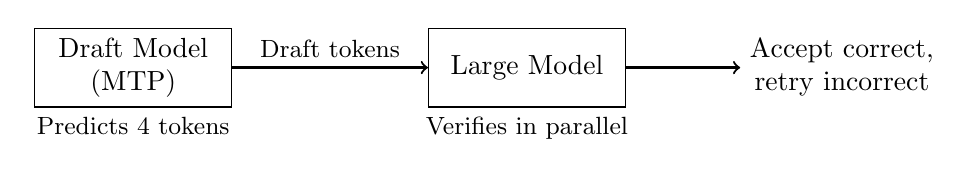
\begin{tikzpicture}
    % Draft Model
    \node[draw, rectangle, minimum width=2.5cm, minimum height=1cm, align=center] (draft) at (0,0) {Draft Model\\(MTP)};
    \node[anchor=north] at (draft.south) {\small Predicts 4 tokens};
    
    % Large Model
    \node[draw, rectangle, minimum width=2.5cm, minimum height=1cm] (verify) at (5,0) {Large Model};
    \node[anchor=north] at (verify.south) {\small Verifies in parallel};
    
    % Result
    \node[align=center] (result) at (9,0) {Accept correct,\\retry incorrect};
    
    % Arrows
    \draw[->, thick] (draft.east) -- (verify.west) node[midway, above] {\small Draft tokens};
    \draw[->, thick] (verify.east) -- (result.west);
\end{tikzpicture}
\caption{Speculative decoding workflow using Multi-Token Prediction}
\end{figure}

\paragraph{Speed Gains:}
If the draft model is right 75\% of the time and generates 4 tokens:
\begin{itemize}
    \item \textbf{Expected accepted:} $0.75 \times 4 = 3$ tokens per verification
    \item \textbf{Cost:} 1 draft forward pass + 1 verification pass
    \item \textbf{Speedup:} $\approx$ 3× compared to standard generation
\end{itemize}

\paragraph{DeepSeek's Choice:}
Interestingly, DeepSeek V3 explicitly chose \textit{not} to use speculative decoding during inference. As stated in their paper:

\begin{quote}
\textit{``Our MTP strategy mainly aims to improve the performance of the main model. During inference, we can directly discard the MTP modules and the main model can function independently and normally."}
\end{quote}

They used MTP purely for its training benefits (densification, data efficiency, planning), not for inference speedup. However, they note that the MTP modules could be repurposed for speculative decoding if desired.

\subsection{How DeepSeek Implemented Multi-Token Prediction}

Now that we understand \textit{why} Multi-Token Prediction is beneficial, let us examine \textit{how} DeepSeek implemented it. Their implementation differs from the original Meta paper in one crucial aspect: \textbf{maintaining causality between predictions}.

\subsubsection{The Original Approach: Independent Predictions}

The original Multi-Token Prediction paper (Meta, 2024) used independent output heads:

\begin{figure}[h]
\centering
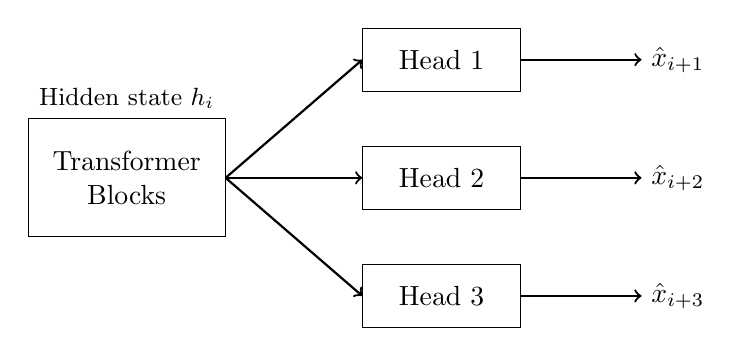
\begin{tikzpicture}
    % Main model
    \node[draw, rectangle, minimum width=2.5cm, minimum height=1.5cm, align=center] (main) at (0,0) {Transformer\\Blocks};
    \node[anchor=south] at (main.north) {\small Hidden state $h_i$};
    
    % Three heads at different heights
    \node[draw, rectangle, minimum width=2cm, minimum height=0.8cm] (head1) at (4, 1.5) {Head 1};
    \node[draw, rectangle, minimum width=2cm, minimum height=0.8cm] (head2) at (4, 0) {Head 2};
    \node[draw, rectangle, minimum width=2cm, minimum height=0.8cm] (head3) at (4, -1.5) {Head 3};
    
    % Predictions
    \node (pred1) at (7, 1.5) {$\hat{x}_{i+1}$};
    \node (pred2) at (7, 0) {$\hat{x}_{i+2}$};
    \node (pred3) at (7, -1.5) {$\hat{x}_{i+3}$};
    
    % Arrows from main to heads
    \draw[->, thick] (main.east) -- (head1.west);
    \draw[->, thick] (main.east) -- (head2.west);
    \draw[->, thick] (main.east) -- (head3.west);
    
    % Arrows from heads to predictions
    \draw[->, thick] (head1.east) -- (pred1.west);
    \draw[->, thick] (head2.east) -- (pred2.west);
    \draw[->, thick] (head3.east) -- (pred3.west);
\end{tikzpicture}
\caption{Original MTP: Independent predictions from the same hidden state}
\end{figure}

\textbf{Limitation:} Each prediction is made independently. The model doesn't use information from predicting token $i+1$ when predicting token $i+2$. This ignores the sequential nature of language.

\subsubsection{DeepSeek's Innovation: Sequential Predictions with Causal Chain}

DeepSeek introduced a crucial innovation: \textbf{maintain a complete causal chain at each prediction depth}. This means:

\begin{itemize}
    \item Prediction at depth $k=1$ influences prediction at depth $k=2$
    \item Prediction at depth $k=2$ influences prediction at depth $k=3$
    \item Information flows sequentially through the prediction depths
\end{itemize}

As stated in the DeepSeek V3 paper:
\begin{quote}
\textit{``We sequentially predict additional tokens and keep the complete causal chain at each prediction depth."}
\end{quote}

This is a significant departure from independent predictions and leads to better results because the model can use information from earlier predictions to inform later ones. 

\begin{figure}[!h]
    \centering
    \includegraphics[width=0.7\linewidth]{images/ch5_02_mtp.pdf}
    \caption{DeepSeek's MTP: Sequential predictions with causal chain. Hidden states propagate from one depth to the next, creating dependencies between predictions. The green arrows show the causal flow of information.}
    \label{fig:freq-decay}
\end{figure}

\textbf{Key Difference:} Notice the green arrows showing how Hidden State 1 feeds into Head 2, and Hidden State 2 feeds into Head 3. This sequential dependency is DeepSeek's main contribution to Multi-Token Prediction.


\subsubsection{Architecture Overview}

DeepSeek's Multi-Token Prediction architecture consists of:

\begin{enumerate}
    \item \textbf{Shared Transformer Trunk:} The main transformer blocks (T1, T2, ..., TN)
    \item \textbf{Multiple MTP Modules:} One module for each prediction depth
    \item \textbf{Hidden State Propagation:} Hidden states flow from one depth to the next
    \item \textbf{Shared Output Head:} A single unembedding matrix used across all depths
\end{enumerate}

Let us break down how this works for a concrete example.

\subsubsection{Detailed Walkthrough: Predicting Three Tokens Ahead}

Suppose we have:
\begin{itemize}
    \item Input sequence: \texttt{[Artificial, intelligence, is, changing, the, world, right, now]}
    \item Embedding dimension: $d = 8$
    \item Prediction depth: $k = 3$ (predict 3 tokens ahead)
    \item Vocabulary size: $V = 50{,}000$
\end{itemize}

We will trace through what happens for the first input token at position $i=0$ (\texttt{Artificial}).

\paragraph{Step 0: Shared Transformer Processing}

All input tokens pass through the shared transformer blocks:
\begin{equation}
H = \text{Transformer}(X)
\end{equation}

where $X \in \mathbb{R}^{8 \times 8}$ (8 tokens, dimension 8), and $H \in \mathbb{R}^{8 \times 8}$ is the output hidden states.

For token at position $i=0$, we have hidden state $h_0 \in \mathbb{R}^{1 \times 8}$ (first row of $H$).

\paragraph{Step 1: First Prediction (Depth $k=1$)}

To predict token at position $i+1$ (\texttt{intelligence}), we need two inputs:

\begin{enumerate}
    \item \textbf{Hidden state:} $h_0$ from the shared transformer (shape: $1 \times 8$)
    \item \textbf{Input embedding:} Embedding of the target position $i+1$ (shape: $1 \times 8$)
\end{enumerate}

\textbf{Operations in Head 1:}

\begin{enumerate}
    \item \textbf{RMS Normalization:}
    \begin{align}
    \tilde{h}_0 &= \text{RMSNorm}(h_0) \\
    \tilde{e}_1 &= \text{RMSNorm}(e_1)
    \end{align}
    where $e_1$ is the input embedding at position $i+1$.
    
    \item \textbf{Concatenation:}
    \begin{equation}
    c_1 = [\tilde{h}_0; \tilde{e}_1] \in \mathbb{R}^{1 \times 16}
    \end{equation}
    Merge the normalized hidden state and embedding.
    
    \item \textbf{Linear Projection:}
    \begin{equation}
    h'_1 = c_1 \cdot M_1 \in \mathbb{R}^{1 \times 8}
    \end{equation}
    where $M_1 \in \mathbb{R}^{16 \times 8}$ is the projection matrix. This brings us back to dimension 8.
    
    \item \textbf{Transformer Layer:}
    \begin{equation}
    h_1 = \text{TransformerBlock}(h'_1) \in \mathbb{R}^{1 \times 8}
    \end{equation}
    Pass through a dedicated transformer block for this depth.
    
    \item \textbf{Output Prediction:}
    \begin{equation}
    \text{logits}_1 = h_1 \cdot W_{\text{unbed}} \in \mathbb{R}^{1 \times 50000}
    \end{equation}
    where $W_{\text{unbed}}$ is the shared unembedding matrix.
    
    Predict: $\hat{x}_{i+1} = \arg\max(\text{logits}_1)$
\end{enumerate}

\paragraph{Step 2: Second Prediction (Depth $k=2$)}

Now we predict token at position $i+2$ (\texttt{is}). Crucially, we use $h_1$ (the hidden state from depth $k=1$) as input:

\begin{enumerate}
    \item \textbf{Inputs:}
    \begin{itemize}
        \item Hidden state: $h_1$ from depth $k=1$ (shape: $1 \times 8$)
        \item Input embedding: $e_2$ at position $i+2$ (shape: $1 \times 8$)
    \end{itemize}
    
    \item \textbf{Operations:} Same as Head 1
    \begin{align}
    \tilde{h}_1 &= \text{RMSNorm}(h_1) \\
    \tilde{e}_2 &= \text{RMSNorm}(e_2) \\
    c_2 &= [\tilde{h}_1; \tilde{e}_2] \in \mathbb{R}^{1 \times 16} \\
    h'_2 &= c_2 \cdot M_2 \in \mathbb{R}^{1 \times 8} \\
    h_2 &= \text{TransformerBlock}(h'_2) \in \mathbb{R}^{1 \times 8} \\
    \text{logits}_2 &= h_2 \cdot W_{\text{unbed}} \in \mathbb{R}^{1 \times 50000}
    \end{align}
    
    Predict: $\hat{x}_{i+2} = \arg\max(\text{logits}_2)$
\end{enumerate}

\paragraph{Step 3: Third Prediction (Depth $k=3$)}

Finally, predict token at position $i+3$ (\texttt{changing}) using $h_2$ from depth $k=2$:

\begin{align}
\tilde{h}_2 &= \text{RMSNorm}(h_2) \\
\tilde{e}_3 &= \text{RMSNorm}(e_3) \\
c_3 &= [\tilde{h}_2; \tilde{e}_3] \\
h'_3 &= c_3 \cdot M_3 \\
h_3 &= \text{TransformerBlock}(h'_3) \\
\text{logits}_3 &= h_3 \cdot W_{\text{unbed}}
\end{align}

Predict: $\hat{x}_{i+3} = \arg\max(\text{logits}_3)$

\paragraph{Key Observations:}

\begin{enumerate}
    \item \textbf{Sequential Flow:} $h_0 \rightarrow h_1 \rightarrow h_2 \rightarrow h_3$
    \item \textbf{Causal Chain:} Each prediction influences the next through hidden states
    \item \textbf{Shared Unembedding:} All depths use the same $W_{\text{unbed}}$ matrix
    \item \textbf{Dedicated Transformers:} Each depth has its own transformer block
    \item \textbf{Dedicated Projections:} Each depth has its own $M_k$ projection matrix
\end{enumerate}

\subsubsection{Loss Computation}

For each input token position, we have $k$ predictions. The total loss is the sum of cross-entropy losses at each depth:

\begin{equation}
\mathcal{L}_{\text{total}} = \sum_{i=0}^{n-k} \sum_{j=1}^{k} \mathcal{L}_{\text{CE}}(\text{logits}_{i,j}, x_{i+j})
\end{equation}

where:
\begin{itemize}
    \item $n$ is the sequence length
    \item $k$ is the prediction depth
    \item $\mathcal{L}_{\text{CE}}$ is cross-entropy loss
    \item $\text{logits}_{i,j}$ are the predicted logits for position $i$ at depth $j$
    \item $x_{i+j}$ is the actual token at position $i+j$
\end{itemize}

For our example with token $i=0$ and $k=3$:
\begin{align}
\mathcal{L}_{i=0} &= \mathcal{L}_{\text{CE}}(\text{logits}_1, \texttt{intelligence}) \\
&\quad + \mathcal{L}_{\text{CE}}(\text{logits}_2, \texttt{is}) \\
&\quad + \mathcal{L}_{\text{CE}}(\text{logits}_3, \texttt{changing})
\end{align}

This loss is then summed across all input positions to get the total batch loss.

\subsubsection{Boundary Handling}

An important implementation detail: what happens at sequence boundaries?

For a sequence of length $n$ with prediction depth $k$:
\begin{itemize}
    \item Tokens at positions $0$ to $n-k-1$ can make all $k$ predictions
    \item Tokens at positions $n-k$ to $n-1$ cannot make all predictions (would exceed sequence length)
\end{itemize}

\textbf{Solution:} Simply skip predictions that would exceed the sequence boundary. For example, if $n=8$ and $k=3$:
\begin{itemize}
    \item Token at $i=5$ can predict $i+1, i+2, i+3$ (positions 6, 7, 8) ✓
    \item Token at $i=6$ can only predict $i+1, i+2$ (positions 7, 8) ✓
    \item Token at $i=7$ can only predict $i+1$ (position 8) ✓
\end{itemize}

\subsection{Mathematical Formulation}

Let us now formalize DeepSeek's Multi-Token Prediction in mathematical notation, following their paper.

\subsubsection{Notation}

\begin{itemize}
    \item $H_i \in \mathbb{R}^d$: Hidden state at position $i$ from shared transformer
    \item $e_i \in \mathbb{R}^d$: Input embedding at position $i$
    \item $k$: Prediction depth (number of future tokens to predict)
    \item $h_i^{(k)} \in \mathbb{R}^d$: Hidden state for position $i$ at prediction depth $k$
    \item $M_k \in \mathbb{R}^{2d \times d}$: Projection matrix for depth $k$
    \item $T_k$: Transformer layer for depth $k$
    \item $W_{\text{unbed}} \in \mathbb{R}^{d \times V}$: Shared unembedding matrix
\end{itemize}

\subsubsection{Forward Pass Equations}

For prediction depth $k$, given input position $i$:

\begin{align}
h_i^{(0)} &= H_i \label{eq:mtp_init} \\
\tilde{h}_i^{(k-1)} &= \text{RMSNorm}(h_i^{(k-1)}) \label{eq:mtp_norm_h} \\
\tilde{e}_{i+k} &= \text{RMSNorm}(e_{i+k}) \label{eq:mtp_norm_e} \\
c_i^{(k)} &= [\tilde{h}_i^{(k-1)}; \tilde{e}_{i+k}] \label{eq:mtp_concat} \\
h'^{(k)}_i &= c_i^{(k)} \cdot M_k \label{eq:mtp_proj} \\
h_i^{(k)} &= T_k(h'^{(k)}_i) \label{eq:mtp_transform} \\
\text{logits}_i^{(k)} &= h_i^{(k)} \cdot W_{\text{unbed}} \label{eq:mtp_logits}
\end{align}

\paragraph{Explanation of Each Step:}

\begin{itemize}
    \item \textbf{Equation \eqref{eq:mtp_init}:} Initialize with hidden state from shared transformer
    \item \textbf{Equations \eqref{eq:mtp_norm_h}-\eqref{eq:mtp_norm_e}:} Normalize both inputs (RMS normalization)
    \item \textbf{Equation \eqref{eq:mtp_concat}:} Concatenate normalized hidden state and embedding
    \item \textbf{Equation \eqref{eq:mtp_proj}:} Project from $2d$ back to $d$ dimensions
    \item \textbf{Equation \eqref{eq:mtp_transform}:} Apply transformer layer for this depth
    \item \textbf{Equation \eqref{eq:mtp_logits}:} Compute logits over vocabulary
\end{itemize}

\subsubsection{Loss Function}

The total Multi-Token Prediction loss is:

\begin{equation}
\mathcal{L}_{\text{MTP}} = \frac{1}{n} \sum_{i=0}^{n-1} \sum_{j=1}^{\min(k, n-i)} \lambda_j \cdot \mathcal{L}_{\text{CE}}(\text{logits}_i^{(j)}, x_{i+j})
\end{equation}

where:
\begin{itemize}
    \item $n$ is the sequence length
    \item $k$ is the maximum prediction depth
    \item $\lambda_j$ is an optional weighting factor for depth $j$ (typically set to 1)
    \item $\min(k, n-i)$ handles boundary cases
\end{itemize}

DeepSeek uses equal weighting ($\lambda_j = 1$ for all $j$), giving equal importance to all prediction depths.

\subsection{Key Design Decisions}

Several important design decisions make DeepSeek's MTP implementation effective:

\subsubsection{1. Shared Unembedding Matrix}

All prediction depths share the same unembedding matrix $W_{\text{unbed}}$. This:
\begin{itemize}
    \item \textbf{Reduces parameters:} No need for $k$ separate output matrices
    \item \textbf{Consistency:} Ensures predictions use the same vocabulary representation
    \item \textbf{Efficiency:} Single matrix can be optimized and cached
\end{itemize}

\subsubsection{2. Separate Transformer Layers per Depth}

Each depth $k$ has its own transformer layer $T_k$. This:
\begin{itemize}
    \item \textbf{Specialization:} Each layer can learn depth-specific patterns
    \item \textbf{Flexibility:} Different depths may require different processing
    \item \textbf{Causality:} Allows information flow between depths
\end{itemize}

\subsubsection{3. RMS Normalization}

Both hidden states and embeddings are normalized before concatenation:
\begin{itemize}
    \item \textbf{Stability:} Prevents one input from dominating
    \item \textbf{Scale invariance:} Makes training more stable
    \item \textbf{Consistency:} Standard practice in modern LLMs
\end{itemize}

\subsubsection{4. Causal Hidden State Chain}

Hidden states flow: $h_0 \rightarrow h_1 \rightarrow h_2 \rightarrow \cdots \rightarrow h_k$

This causal chain is DeepSeek's main contribution to MTP:
\begin{itemize}
    \item \textbf{Sequential reasoning:} Later predictions build on earlier ones
    \item \textbf{Consistency:} Predictions are mutually consistent
    \item \textbf{Richer gradients:} Errors propagate through the chain
\end{itemize}

\subsection{Training vs. Inference}

An important aspect of DeepSeek's MTP implementation is the distinction between training and inference:

\subsubsection{During Training (Pre-training)}

DeepSeek uses the \textit{full} Multi-Token Prediction architecture:
\begin{itemize}
    \item All $k$ prediction depths are active
    \item Model receives dense training signal
    \item Hidden states propagate through MTP modules
    \item Loss computed across all depths
\end{itemize}

\textbf{Benefits exploited:}
\begin{enumerate}
    \item Densification of training signals
    \item Improved data efficiency
    \item Better planning through implicit weighting
\end{enumerate}

\subsubsection{During Inference}

DeepSeek \textit{discards} the MTP modules entirely:
\begin{itemize}
    \item Only the main model (shared transformer) is used
    \item Standard single-token prediction
    \item No speculative decoding
    \item MTP parameters are not loaded
\end{itemize}

\textbf{Rationale:}
\begin{itemize}
    \item \textbf{Simplicity:} Standard autoregressive generation is well-understood
    \item \textbf{Compatibility:} Works with existing inference infrastructure
    \item \textbf{Sufficient quality:} Training benefits carry over to the main model
\end{itemize}

As stated in their paper:
\begin{quote}
\textit{``During inference, we can directly discard the MTP modules and the main model can function independently and normally."}
\end{quote}

However, they note that the MTP modules \textit{could} be repurposed for speculative decoding if faster inference is desired:
\begin{quote}
\textit{``Additionally, we can also repurpose these MTP modules for speculative decoding."}
\end{quote}

This design decision reflects DeepSeek's pragmatic approach: use MTP to improve training, but keep inference simple and standard.

\subsection{Summary: The Third Pillar}

Multi-Token Prediction completes DeepSeek's three-pillar architecture:

\begin{enumerate}
    \item \textbf{MLA:} Reduces memory cost through KV cache compression (4-8× savings)
    \item \textbf{MoE:} Increases model capacity through sparse expert routing (3× parameter efficiency)
    \item \textbf{MTP:} Improves training through dense supervision signals (richer representations)
\end{enumerate}

Together, these innovations create a model that is:
\begin{itemize}
    \item \textbf{Memory-efficient:} Can handle long contexts with limited memory
    \item \textbf{High-capacity:} Has many parameters but uses them sparsely
    \item \textbf{Well-trained:} Learns richer representations from the same data
    \item \textbf{Practical:} Uses standard inference despite advanced training
\end{itemize}

The beauty of MTP is its simplicity: predict more tokens, get better training. Yet this simple idea, combined with DeepSeek's innovation of maintaining causal chains, leads to measurable improvements in model quality. In the next section, we will see how Multi-Token Prediction is implemented in our codebase.

\section{Coding Multi-Token Prediction}

Having explored the theory and architecture of Multi-Token Prediction, we now examine its practical implementation. Our MTP implementation follows the DeepSeek-V3 architecture exactly, with sequential prediction heads that maintain causal information flow between depths.

The implementation consists of three key components:

\begin{enumerate}
    \item \textbf{RMSNorm Layer}: Normalizes hidden states and embeddings before concatenation
    \item \textbf{MultiTokenPrediction Module}: Implements sequential prediction heads with causal flow
    \item \textbf{Loss Computation}: Accumulates cross-entropy losses across all positions and depths
\end{enumerate}

\subsection{RMSNorm: Stabilizing Input Concatenation}

Before concatenating hidden states and token embeddings in each prediction head, we apply Root Mean Square normalization to ensure both inputs have similar scales:

\begin{minted}{python}
class RMSNorm(nn.Module):
    """
    Root Mean Square Layer Normalization.
    
    RMSNorm is used before concatenating hidden states and embeddings in each MTP head.
    It normalizes input by dividing by the RMS (root mean square) of the input elements.
    
    Formula: RMSNorm(x) = x / sqrt(mean(x^2) + eps)
    """
    
    def __init__(self, d_model: int, eps: float = 1e-8):
        super().__init__()
        self.eps = eps
    
    def forward(self, x: torch.Tensor) -> torch.Tensor:
        """Apply RMSNorm to input tensor."""
        # Calculate RMS: sqrt of mean of squares
        rms = torch.sqrt(x.pow(2).mean(dim=-1, keepdim=True) + self.eps)
        # Normalize by dividing by RMS
        return x / rms
\end{minted}

This normalization prevents one component from dominating the concatenated vector and stabilizes training.

\subsection{MultiTokenPrediction Module}

The core MTP implementation creates sequential prediction heads where each head builds on the previous head's hidden state:

\begin{minted}{python}
class MultiTokenPrediction(nn.Module):
    """
    Multi-Token Prediction mechanism for DeepSeek training.
    
    MTP predicts multiple future tokens (depth D) at each input position using
    sequential transformer blocks. Each head predicts one token into the future,
    with causality maintained by passing hidden states between heads.
    
    For an input sequence of length T:
    - At position i, predict tokens at positions i+1, i+2, ..., i+D
    - Use D sequential heads, each building on the previous head's output
    - Total predictions: (T-D) * D tokens
    """
    
    def __init__(self, d_model: int, vocab_size: int, num_heads: int, nhead: int, cfg: dict):
        super().__init__()
        self.d_model = d_model
        self.vocab_size = vocab_size
        self.num_heads = num_heads  # Depth D
        
        # Shared normalization layer for hidden states and embeddings
        self.rmsnorm = RMSNorm(d_model)
        
        # Embedding layer (shared with main model through weight tying)
        self.embed = nn.Embedding(vocab_size, d_model)
        
        # Output projection (shared with embedding through weight tying)
        self.unembed = nn.Linear(d_model, vocab_size, bias=False)
        # Weight tying: share weights between embedding and output projection
        self.unembed.weight = self.embed.weight
        
        # One linear projection per head: projects concatenated (2*d_model) back to d_model
        # Each head needs its own projection to learn different future predictions
        self.projections = nn.ModuleList([
            nn.Linear(2 * d_model, d_model) for _ in range(num_heads)
        ])
        
        # One transformer block per head: processes projected features
        # Each transformer learns to predict a different step into the future
        self.transformers = nn.ModuleList([
            TransformerBlock(cfg) for _ in range(num_heads)
        ])
\end{minted}

\subsection{Forward Pass: Sequential Prediction with Causal Flow}

The forward pass implements DeepSeek's key innovation: maintaining causal information flow between prediction depths:

\begin{minted}{python}
    def forward(self, token_ids: torch.Tensor, init_hidden: torch.Tensor = None) -> torch.Tensor:
        """
        Forward pass for Multi-Token Prediction.
        
        Process:
        1. Get token embeddings for entire sequence
        2. For each position i where i + D < T:
            a. Initialize base hidden state (from init_hidden or embeddings)
            b. For each head k (k=0 to D-1):
                - Get future token embedding at position i+(k+1)
                - RMSNorm hidden state and embedding
                - Concatenate and project to d_model
                - Pass through transformer block
                - Generate logits for next token
                - Update hidden state for next head (causal flow)
        3. Stack all predictions into (batch, T-D, D, vocab_size) tensor
        
        Returns:
            logits: Predictions of shape (batch, T-D, D, vocab_size)
                   logits[b, i, k, :] = predicted logits for token at position i+(k+1)
        """
        batch_size, seq_len = token_ids.shape
        
        # Get token embeddings for entire sequence: (batch, seq_len, d_model)
        embeds = self.embed(token_ids)
        
        # Initialize base hidden states
        if init_hidden is None:
            h0_seq = embeds  # (batch, seq_len, d_model)
        else:
            h0_seq = init_hidden  # (batch, seq_len, d_model)
        
        # List to collect predictions for each valid position
        outputs = []
        
        # Calculate maximum valid starting position
        # For position i, we predict tokens at i+1, i+2, ..., i+D
        # So we need i + D < seq_len, which means i < seq_len - D
        max_i = seq_len - self.num_heads - 1
        
        # Iterate over positions where we can predict D tokens into the future
        for i in range(0, max_i):
            # Get base hidden state at position i: (batch, d_model)
            h_prev = h0_seq[:, i, :]
            
            # Collect logits for all D prediction heads at this position
            logits_k = []
            
            # For each prediction head k, predict token at position i+(k+1)
            for k in range(self.num_heads):
                # Future position we're predicting
                future_pos = i + (k + 1)
                
                # Get embedding of the token at the target future position
                tok_embed = embeds[:, future_pos, :]  # (batch, d_model)
                
                # Step 1: RMS-normalize both hidden state and token embedding
                h_norm = self.rmsnorm(h_prev)      # (batch, d_model)
                e_norm = self.rmsnorm(tok_embed)   # (batch, d_model)
                
                # Step 2: Concatenate normalized vectors
                merged = torch.cat([h_norm, e_norm], dim=-1)  # (batch, 2*d_model)
                
                # Step 3: Project back to d_model
                proj = self.projections[k](merged)  # (batch, d_model)
                
                # Step 4: Pass through transformer block
                # Add sequence dimension for transformer: (batch, 1, d_model)
                x = proj.unsqueeze(1)
                x = self.transformers[k](x)  # (batch, 1, d_model)
                h_curr = x.squeeze(1)  # (batch, d_model)
                
                # Step 5: Project to vocabulary to get logits
                logits = self.unembed(h_curr)  # (batch, vocab_size)
                logits_k.append(logits)
                
                # Step 6: Update hidden state for next head (causal flow)
                h_prev = h_curr
            
            # Stack predictions for all D heads at position i: (batch, D, vocab_size)
            logits_k = torch.stack(logits_k, dim=1)
            outputs.append(logits_k)
        
        # Stack predictions for all positions: (batch, T-D, D, vocab_size)
        out = torch.stack(outputs, dim=1)
        
        return out
\end{minted}

\paragraph{Key Implementation Details:}

\begin{itemize}
    \item \textbf{Causal Flow:} Each head's output becomes the next head's input (\texttt{h\_prev = h\_curr})
    \item \textbf{Weight Tying:} Embedding and unembedding matrices are shared (\texttt{self.unembed.weight = self.embed.weight})
    \item \textbf{Boundary Handling:} Only predict from positions where all future tokens exist (\texttt{max\_i = seq\_len - self.num\_heads - 1})
    \item \textbf{Sequential Processing:} Each depth has its own projection and transformer block
\end{itemize}

\subsection{Loss Computation}

The MTP loss accumulates cross-entropy losses across all positions and depths:

\begin{minted}{python}
def compute_mtp_loss(logits: torch.Tensor, targets: torch.Tensor) -> torch.Tensor:
    """
    Compute the Multi-Token Prediction loss.
    
    The MTP loss is computed by:
    1. For each position i and each depth k:
       - Compare logits[i, k] with targets[i + k + 1]
       - Compute cross-entropy loss
    2. Sum all losses and normalize by (L * D)
       where L is number of positions, D is depth
    
    Args:
        logits: Model predictions of shape (batch, L, D, vocab_size)
                where L = T-D positions, D = depth
        targets: Target token IDs of shape (batch, T) where T is full sequence length
    
    Returns:
        loss: Scalar tensor containing the averaged MTP loss
    
    Mathematical formulation:
        loss = (1/(L*D)) * Σ_i Σ_k CrossEntropy(logits[i,k], targets[i+k+1])
    """
    batch_size, L, D, vocab_size = logits.shape
    _, seq_len = targets.shape
    
    # Verify dimensions are compatible
    assert L == seq_len - D - 1, f"Expected L={seq_len - D - 1}, got L={L}"
    
    # Initialize total loss
    loss = 0.0
    
    # Double loop over positions (i) and depth (k)
    for i in range(L):
        for k in range(D):
            # Get predicted logits for position i, depth k
            logit_ik = logits[:, i, k, :]  # (batch, vocab_size)
            
            # Get target token at position i + (k+1)
            target_ik = targets[:, i + (k + 1)]  # (batch,)
            
            # Compute cross-entropy loss for this (i, k) pair
            loss += F.cross_entropy(logit_ik, target_ik)
    
    # Normalize by total number of predictions (L * D)
    loss = loss / (L * D)
    
    return loss
\end{minted}

This ensures each prediction contributes equally to the total loss, with normalization making the magnitude comparable to standard next-token prediction.

\subsection{Summary: The Complete MTP Implementation}

Our Multi-Token Prediction implementation provides the core components needed to integrate MTP into any transformer architecture:

\begin{itemize}
    \item \textbf{RMSNorm}: Stabilizes concatenation of hidden states and embeddings
    \item \textbf{MultiTokenPrediction Module}: Implements sequential prediction heads with causal flow
    \item \textbf{Loss Computation}: Accumulates cross-entropy losses across all positions and depths
\end{itemize}

\paragraph{Key Features:}

\begin{enumerate}
    \item \textbf{Causal Information Flow:} Each prediction head builds on the previous head's output, maintaining sequential dependencies
    \item \textbf{Weight Tying:} Embedding and unembedding matrices are shared to reduce parameters
    \item \textbf{Boundary Handling:} Only predicts from positions where all future tokens exist
    \item \textbf{Flexible Depth:} Configurable number of future tokens to predict (typically 3)
\end{enumerate}

\paragraph{Benefits Realized:}

\begin{itemize}
    \item \textbf{Densified Training Signals:} $(T-D) \times D$ predictions vs. $T-1$ standard predictions
    \item \textbf{Improved Data Efficiency:} Learn more from each training batch
    \item \textbf{Sequential Reasoning:} Causal chains through prediction heads
    \item \textbf{Modular Design:} Easy to integrate into existing transformer architectures
\end{itemize}

Multi-Token Prediction completes DeepSeek's three-pillar architecture, working alongside MLA (memory efficiency) and MoE (parameter efficiency) to provide training efficiency. The implementation follows the DeepSeek-V3 architecture exactly, providing 2-3× more training signals from the same data while maintaining the sequential dependencies that make MTP effective.

For the complete implementation details, for training code refer to the codebase \psnote{TODO: add link to github here}, which includes comprehensive docstrings and comments explaining each component. 

With our understanding of DeepSeek's three core innovations—MLA for memory efficiency, MoE for parameter efficiency, and MTP for training efficiency—we now turn to a critical practical consideration: how to actually deploy these massive models in production. In the next section, we'll explore quantization techniques that make it possible to run billion-parameter models on consumer hardware without sacrificing too much performance.

\section{Quantization: The Final Pillar of DeepSeek}

This section explores quantization not as a post-training optimization, but as a fundamental training methodology. DeepSeek-V3 was trained using FP8 (8-bit floating point) precision from the ground up, achieving near-identical performance to traditional BF16 training while dramatically reducing memory requirements and computational costs.

\subsection{Understanding Quantization: Why It Matters}

Before diving into DeepSeek's innovations, let us establish what quantization means and why it is essential for large language models.

\subsubsection{The Memory Challenge}

Every parameter in a neural network occupies memory. The amount of memory a parameter requires depends on how we \textit{represent} it numerically. Consider a simple parameter value like $\pi = 3.14159...$

In the most common representation, \textbf{floating point 32-bit (FP32)}, this value is stored using 32 bits:

\begin{itemize}
    \item \textbf{1 bit} for the sign (positive or negative)
    \item \textbf{8 bits} for the exponent (determines the range)
    \item \textbf{23 bits} for the mantissa (determines the precision)
\end{itemize}

This representation provides:
\begin{itemize}
    \item \textbf{Range:} $\pm 3.4 \times 10^{38}$
    \item \textbf{Precision:} Approximately 7 decimal digits
\end{itemize}

For a model with 671 billion parameters like DeepSeek-V3, storing all parameters in FP32 would require:
\begin{equation}
671 \times 10^9 \text{ parameters} \times 4 \text{ bytes/parameter} = 2.68 \text{ TB}
\end{equation}

This is prohibitively expensive for both training and inference. The situation becomes even more challenging when we consider:

\begin{enumerate}
    \item \textbf{Optimizer States:} AdamW optimizer maintains first and second moments for each parameter, multiplying memory requirements by 3×
    \item \textbf{Gradients:} During training, we must store gradients for backpropagation
    \item \textbf{Activations:} Intermediate layer outputs must be cached for backward pass
    \item \textbf{KV Cache:} For inference, attention mechanisms require caching keys and values
\end{enumerate}

\subsubsection{The Quantization Solution}

Quantization reduces memory requirements by representing parameters with fewer bits. The key insight is that we can often reduce precision without significantly degrading model performance.

\paragraph{Common Precision Formats}

\begin{table}[h]
\centering
\begin{tabular}{|l|c|c|c|c|}
\hline
\textbf{Format} & \textbf{Bits} & \textbf{Sign} & \textbf{Exponent} & \textbf{Mantissa} \\
\hline
FP32 & 32 & 1 & 8 & 23 \\
FP16 & 16 & 1 & 5 & 10 \\
BF16 & 16 & 1 & 8 & 7 \\
FP8 (E4M3) & 8 & 1 & 4 & 3 \\
FP8 (E5M2) & 8 & 1 & 5 & 2 \\
INT8 & 8 & 1 & - & 7 (integer) \\
\hline
\end{tabular}
\caption{Common numerical precision formats used in deep learning}
\end{table}

\begin{itemize}
    \item \textbf{FP16 (Half Precision):} Reduces bits from 32 to 16, cutting memory in half. However, the reduced exponent bits limit the representable range to $\pm 65,504$.

    \item \textbf{BF16 (Brain Float 16):} Maintains the same exponent bits as FP32 (range of $\pm 3.4 \times 10^{38}$) but reduces mantissa bits. This preserves the ability to represent very large and very small numbers, making it more stable for training.

    \item \textbf{FP8:} The most aggressive floating-point quantization. Two variants exist:
    \begin{itemize}
        \item \textbf{E4M3:} 4 exponent bits, 3 mantissa bits—prioritizes precision
        \item \textbf{E5M2:} 5 exponent bits, 2 mantissa bits—prioritizes range
    \end{itemize}

    \item \textbf{INT8:} Represents only integers in the range $[-127, 127]$, using no exponent bits.
\end{itemize}


\subsubsection{The Quantization Process: A Simple Example}

To understand how quantization works, consider converting a set of FP32 values to INT8:

\begin{tcolorbox}[colback=blue!5!white,colframe=blue!75!black,title=Example: FP32 to INT8 Quantization]
Given the FP32 values: $[-7.59, -3.45, 0.82, 5.31, 10.8]$

\textbf{Step 1: Find the scaling factor}
\begin{equation}
\alpha = \max(|\text{values}|) = 10.8
\end{equation}

\textbf{Step 2: Scale and quantize each value}
\begin{equation}
x_{\text{INT8}} = \text{round}\left(\frac{x_{\text{FP32}}}{\alpha} \times 127\right)
\end{equation}

\textbf{Results:}
\begin{align*}
-7.59 &\rightarrow \text{round}\left(\frac{-7.59}{10.8} \times 127\right) = -89 \\
-3.45 &\rightarrow \text{round}\left(\frac{-3.45}{10.8} \times 127\right) = -41 \\
0.82 &\rightarrow \text{round}\left(\frac{0.82}{10.8} \times 127\right) = 10 \\
5.31 &\rightarrow \text{round}\left(\frac{5.31}{10.8} \times 127\right) = 62 \\
10.8 &\rightarrow \text{round}\left(\frac{10.8}{10.8} \times 127\right) = 127
\end{align*}

\textbf{Dequantization (when needed):}
\begin{equation}
x_{\text{FP32}} \approx \frac{x_{\text{INT8}}}{127} \times \alpha
\end{equation}
\end{tcolorbox}

This scaling by the maximum absolute value is crucial—it ensures we fully utilize the available range while preventing overflow. This concept becomes even more important in DeepSeek's fine-grained quantization approach.

\subsubsection{The Trade-off: Memory vs. Accuracy}

Quantization is not free. Reducing precision introduces quantization error:

\begin{equation}
\text{Error} = |x_{\text{original}} - x_{\text{quantized}}|
\end{equation}

However, for large language models, the key empirical finding is that:

\begin{tcolorbox}[colback=blue!5!white,colframe=blue!75!black,title=The Quantization Sweet Spot]
With careful implementation, we can achieve:
\begin{itemize}
    \item \textbf{75\% memory reduction} (FP32 → FP8)
    \item \textbf{<0.25\% increase in training loss} (DeepSeek-V3 result)
\end{itemize}

The memory savings enable larger models, longer context windows, and faster training—benefits that far outweigh the minimal accuracy loss.
\end{tcolorbox}

\subsection{DeepSeek's FP8 Training Framework}

DeepSeek-V3 pushes quantization to its limits by training entirely in FP8 precision. This is not simply applying quantization to a trained model—it requires rethinking the entire training pipeline. DeepSeek's approach consists of five key innovations:

\begin{enumerate}
    \item \textbf{Mixed Precision Framework:} Strategically choosing which operations use FP8 vs. higher precision
    \item \textbf{Fine-Grained Quantization:} Preventing outliers from degrading quantization quality
    \item \textbf{Increased Accumulation Precision:} Maintaining accuracy in matrix multiplications
    \item \textbf{Mantissa over Exponents:} Prioritizing precision over range through E4M3 format
    \item \textbf{Online Quantization:} Computing scaling factors on-the-fly rather than from history
\end{enumerate}

Let us explore each innovation in detail.

\subsection{Innovation 1: Mixed Precision Framework}

The first key insight is that \textit{not all operations benefit equally from quantization}. Some operations are compute-intensive and memory-hungry (ideal for FP8), while others are numerically sensitive and require higher precision.

\subsubsection{The Forward Pass (Fprop)}

Consider a standard linear layer operation:
\begin{equation}
Y = WX + b
\end{equation}

where $X$ is the input, $W$ are weights, and $Y$ is the output.

\paragraph{DeepSeek's Strategy for Forward Pass:}

\begin{enumerate}
    \item \textbf{Inputs ($X$):} Convert from BF16 to FP8 on-the-fly
    \item \textbf{Weights ($W$):} Stored in BF16/FP32, converted to FP8 when needed
    \item \textbf{Computation:} $Y = W_{\text{FP8}} \cdot X_{\text{FP8}}$ executed in FP8
    \item \textbf{Accumulation:} Results initially accumulated in FP32
    \item \textbf{Output ($Y$):} Stored as BF16 for memory efficiency while maintaining range
\end{enumerate}

\begin{tcolorbox}[colback=green!5!white,colframe=green!75!black,title=Why BF16 for Output Storage?]
Brain Float 16 (BF16) is chosen because it:
\begin{itemize}
    \item Maintains the same \textbf{dynamic range} as FP32 ($\pm 3.4 \times 10^{38}$)
    \item Uses only \textbf{16 bits} (half the memory of FP32)
    \item Provides adequate \textbf{precision} (7 mantissa bits) for activations
\end{itemize}
This prevents overflow/underflow issues common in FP16 while achieving 2× memory savings over FP32.
\end{tcolorbox}

\subsubsection{The Backward Pass: Two Gradients}

During backpropagation, we compute two types of gradients:

\paragraph{Activation Gradient (Dgrad):} $\frac{\partial L}{\partial X}$

This gradient flows backward through the network and becomes the gradient for the previous layer. DeepSeek's approach:

\begin{enumerate}
    \item \textbf{Input Gradient:} Arrives from next layer as BF16, converted to FP8
    \item \textbf{Weights:} Converted to FP8 (reusing forward pass quantization)
    \item \textbf{Computation:} $(W_{\text{FP8}})^T \cdot \frac{\partial L}{\partial Y}_{\text{FP8}}$ in FP8
    \item \textbf{Output:} Stored as BF16 for next layer's backward pass
\end{enumerate}

\paragraph{Weight Gradient (Wgrad):} $\frac{\partial L}{\partial W}$

This gradient updates the model's parameters. Since optimization is critical, more care is needed:

\begin{enumerate}
    \item \textbf{Computation:} $X_{\text{FP8}} \cdot \left(\frac{\partial L}{\partial Y}\right)_{\text{FP8}}$ in FP8
    \item \textbf{Accumulation:} Results accumulated in FP32 for precision
    \item \textbf{Storage:} Gradients stored as BF16 before optimizer step
\end{enumerate}

\subsubsection{What Stays in High Precision?}

Not everything can be quantized. DeepSeek maintains original precision (BF16 or FP32) for:

\begin{itemize}
    \item \textbf{Embedding Layers:} Input and output token embeddings
    \item \textbf{Layer Normalization:} RMSNorm operations
    \item \textbf{Attention Computations:} Softmax and attention weights
    \item \textbf{MoE Gating:} Router decisions for expert selection
    \item \textbf{Master Weights:} The authoritative copy of parameters in the optimizer
    \item \textbf{Optimizer States:} Adam's first and second moments
\end{itemize}

\begin{tcolorbox}[colback=yellow!5!white,colframe=yellow!75!black,title=The Mixed Precision Philosophy]
\textbf{Core Principle:} Execute expensive matrix multiplications in FP8 (gaining 2× speedup and 2× memory savings), while keeping numerically sensitive operations in higher precision.

This hybrid approach achieves the best of both worlds: the efficiency of FP8 computation with the stability of higher precision where it matters.
\end{tcolorbox}

\subsection{Innovation 2: Fine-Grained Quantization}

The mixed precision framework tells us \textit{when} to use FP8, but not \textit{how} to quantize effectively. The challenge: \textbf{outliers}.

\subsubsection{The Outlier Problem}

Recall our quantization formula from earlier:
\begin{equation}
x_{\text{quantized}} = \text{round}\left(\frac{x}{\alpha} \times 127\right), \quad \alpha = \max(|x|)
\end{equation}

When a tensor contains an outlier—a single extremely large value—the scaling factor $\alpha$ becomes large, causing all other values to map to a narrow range.

\begin{tcolorbox}[colback=red!5!white,colframe=red!75!black,title=Example: The Outlier Problem]
Consider quantizing these values to INT8: $[1.2, 0.8, 3.4, 2.1, 100.0]$

\textbf{Naive quantization:}
\begin{itemize}
    \item Scaling factor: $\alpha = 100.0$
    \item Results: $[2, 1, 4, 3, 127]$
\end{itemize}

The outlier (100.0) forces all normal values into the range $[1, 4]$, wasting most of the available representational capacity $[-127, 127]$ and losing precision.
\end{tcolorbox}

This problem is pervasive in neural networks: activations often exhibit \textbf{feature outliers}—a few channels with abnormally large magnitudes that dominate the scaling factor.

\subsubsection{The Solution: Fine-Grained Quantization}

DeepSeek's solution is elegant: instead of computing one scaling factor for the entire tensor, compute separate scaling factors for smaller groups of elements.

\paragraph{For Activations (Vectors):} Tile-wise grouping

Activations are typically vectors of shape $(\text{batch}, \text{sequence\_length}, \text{channels})$. DeepSeek groups along the channel dimension:

\begin{equation}
\text{Tile size} = 1 \times 128 \text{ elements}
\end{equation}

Each tile of 128 consecutive channels gets its own scaling factor:

\begin{equation}
\alpha_i = \max(|X_{:, i:i+128}|), \quad i = 0, 128, 256, \ldots
\end{equation}

\paragraph{For Weights (Matrices):} Block-wise grouping

Weight matrices have shape $(\text{in\_features}, \text{out\_features})$. DeepSeek uses block-wise quantization:

\begin{equation}
\text{Block size} = 128 \times 128 \text{ elements}
\end{equation}

Each $128 \times 128$ block gets its own scaling factor:

\begin{equation}
\alpha_{ij} = \max(|W_{i:i+128, j:j+128}|)
\end{equation}

\subsection{Innovation 3: Increased Accumulation Precision}

Fine-grained quantization solves the \textit{input} quantization problem. But there's another challenge: what happens during matrix multiplication itself?

When accumulating many small FP8 numbers, limited precision causes underflow. DeepSeek \textbf{periodically promotes} intermediate results to CUDA Cores for high-precision FP32 accumulation rather than accumulating entirely on Tensor Cores.

\subsection{Innovation 4: Mantissa over Exponents}

DeepSeek uses E4M3 format uniformly (prioritizing precision with 3 mantissa bits) rather than hybrid E4M3/E5M2 approaches. This works because fine-grained quantization's per-group scaling effectively "shares" exponent bits across groups, eliminating the need for extra exponent bits.

\subsection{Innovation 5: Online Quantization}

Instead of using historical scaling factors (delayed quantization), DeepSeek computes scaling factors on-the-fly:

\begin{equation}
\alpha_t = \max(|x_t|)
\end{equation}

This prevents overflow/underflow when distributions shift during training, at minimal computational cost.

\subsection{Summary: The Complete Picture}

DeepSeek's five quantization innovations work synergistically to enable FP8 training with <0.25\% loss degradation:

\begin{enumerate}
    \item \textbf{Mixed Precision:} FP8 for compute-intensive General Matrix-Matrix Multiplication (GEMMs), higher precision for sensitive ops
    \item \textbf{Fine-Grained Quantization:} Per-group scaling isolates outliers
    \item \textbf{Increased Accumulation:} Periodic promotion to FP32 prevents underflow
    \item \textbf{E4M3 Format:} Mantissa bits for precision, groups share exponent range
    \item \textbf{Online Scaling:} Real-time computation prevents distribution shift issues
\end{enumerate}

Combined with MLA (memory efficiency), MoE (parameter efficiency), and MTP (training efficiency), quantization completes DeepSeek's architecture: a model that achieves state-of-the-art performance at dramatically reduced cost.


%%%%%%%%%%%%%%%%%%%%%%%%%%
% Bibliography
\backmatter
\printbibliography[heading=bibintoc]

\end{document}